\section{Mobile Interface}
Design is a crucial topic in developing a mobile application. A key issue when
conceiving a design is thinking that having a "nice-looking" app is enough to achieve it. The first error while approaching the design phase is not to put the user at the centre. When software is intuitive, users have a more pleasant experience and tend to use it again while, if they find difficulties, their painful experience will make them abandon the application.\newline

The first things to understand during the design phase was how users would have moved inside Expire App. We wanted to group the various elements in characterizing our offer by domain, to make as most intuitive as possible
for users to add for eg., a product, or view a recipe. To achieve our objective, we divided the application into five main sections:

\begin{itemize}
    \item \textbf{Recipe screen: } containing the list of recipes based on the products that the user has
    
    \item \textbf{Shopping List screen: } containing lists of products that the user can insert
    
    \item \textbf{Home screen: } containing the list of products that the user has, it gives also the possibility to add new products
    
    \item \textbf{Statistics screen: } containing some statistical infos about the products that the user has (for eg. the quantity of salt in products, quantity of fat, etc..)
    
    \item \textbf{User info screen: } containing profile informations, and gives to the user the possibility to change his/her display name, leave a family, join a family, and logout.
\end{itemize}

To let the user navigate among these sections, we used a Tab selector, which
provides some buttons on the bottom of the display, where each button corresponds to a single screen.\newline

\textbf{Interactive components: } One of the main goal in developing Expire App, is to create a user friendly interface, so our team decided to put particular focus on how interactive elements, like buttons and cards, should behave. To achieve this, as already stated Expire App is developed as well as for different platforms, but also for different screen resolutions and sizes, including landscape versions. Next sections will show the screens related to each of the views listed above.

\subsection{Authentication screen}
The authentication screen, containing the forms to login and register in the service, is the one that appears when the user opens for the first time the application (after an initial onboard screen).
In the login section, as shown in the below figure, if a user is using an iOS device, he/she could also login/register with Apple ID, or even continue without registration (possible also for Android OS users).
In the registration screen, there is also the possibility to register with already having a family ID, in this way once the user enters in the application, on the homepage he/she will have could view the products of all family members.\newline

\vspace*{-0.3cm}
\begin{figure}[H]
  \begin{minipage}{0.5\textwidth}
  \centering
    \includegraphics[width=42.mm,scale=0.9]{./Images//Mobile_mocks/Login.png}
    \vspace*{-0.3cm}
    \caption{Mobile Login page}
    \end{minipage}
\hfill
   \begin{minipage}{0.5\textwidth}
     \centering
     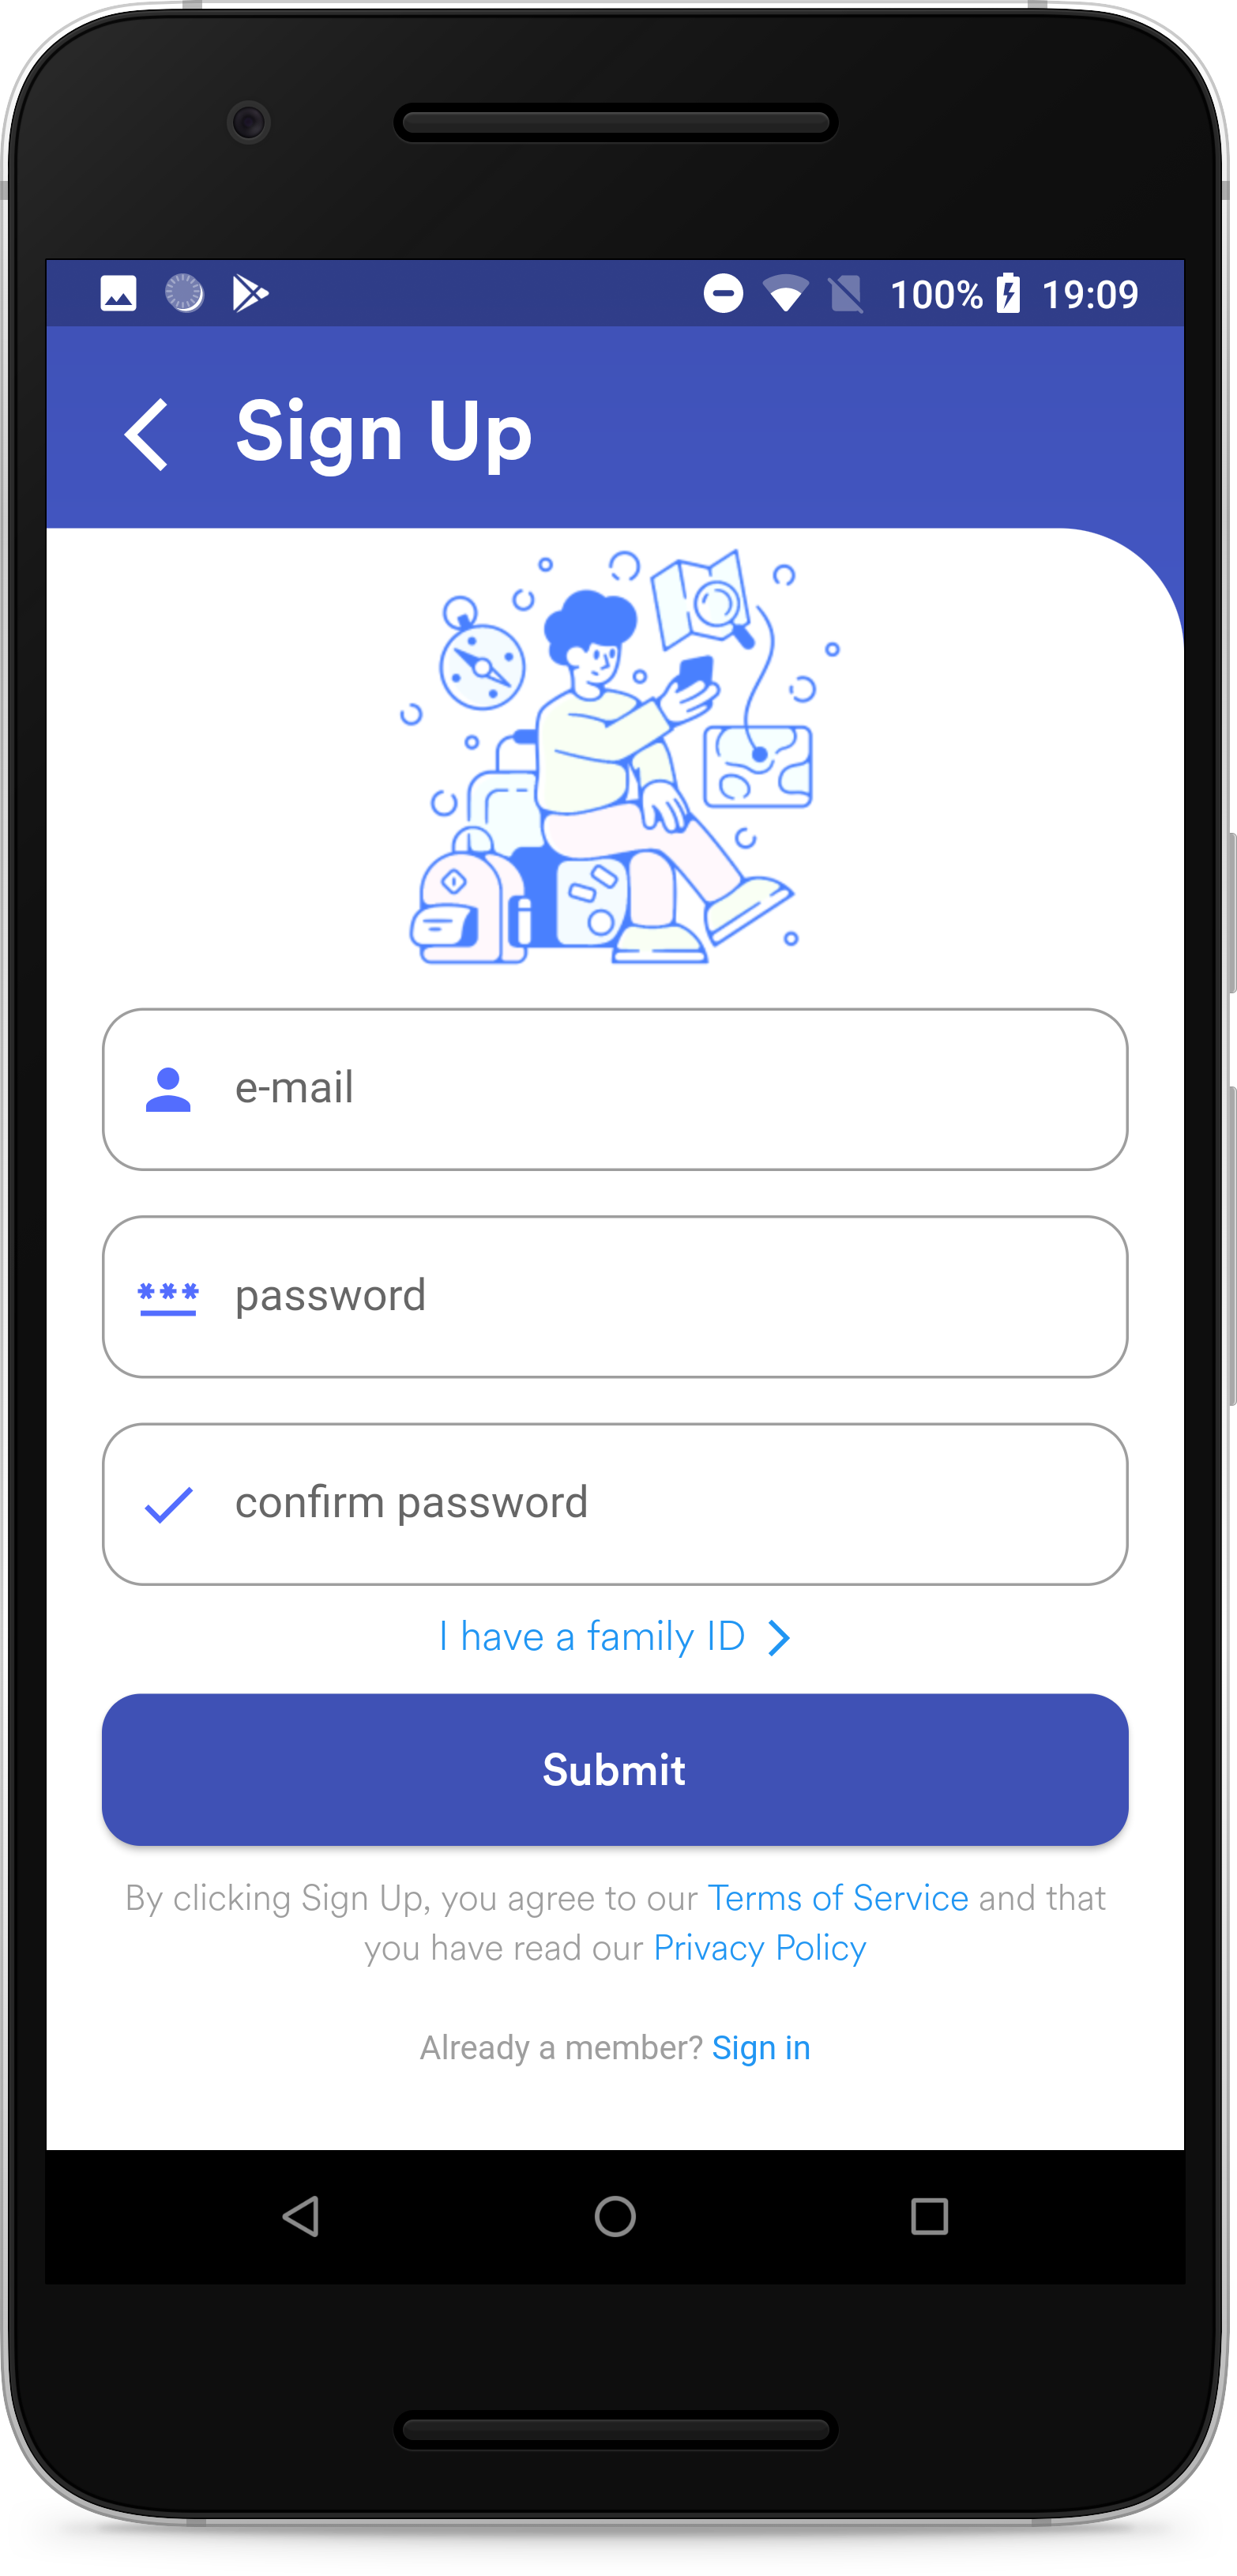
\includegraphics[width=42mm,scale=0.9]{./Images//Mobile_mocks/registration.png}
     \vspace*{-0.3cm}
     \caption{Mobile Registration page}
   \end{minipage}
\end{figure}

\vspace*{-0.3cm}
\begin{figure}[H]
  \centering
    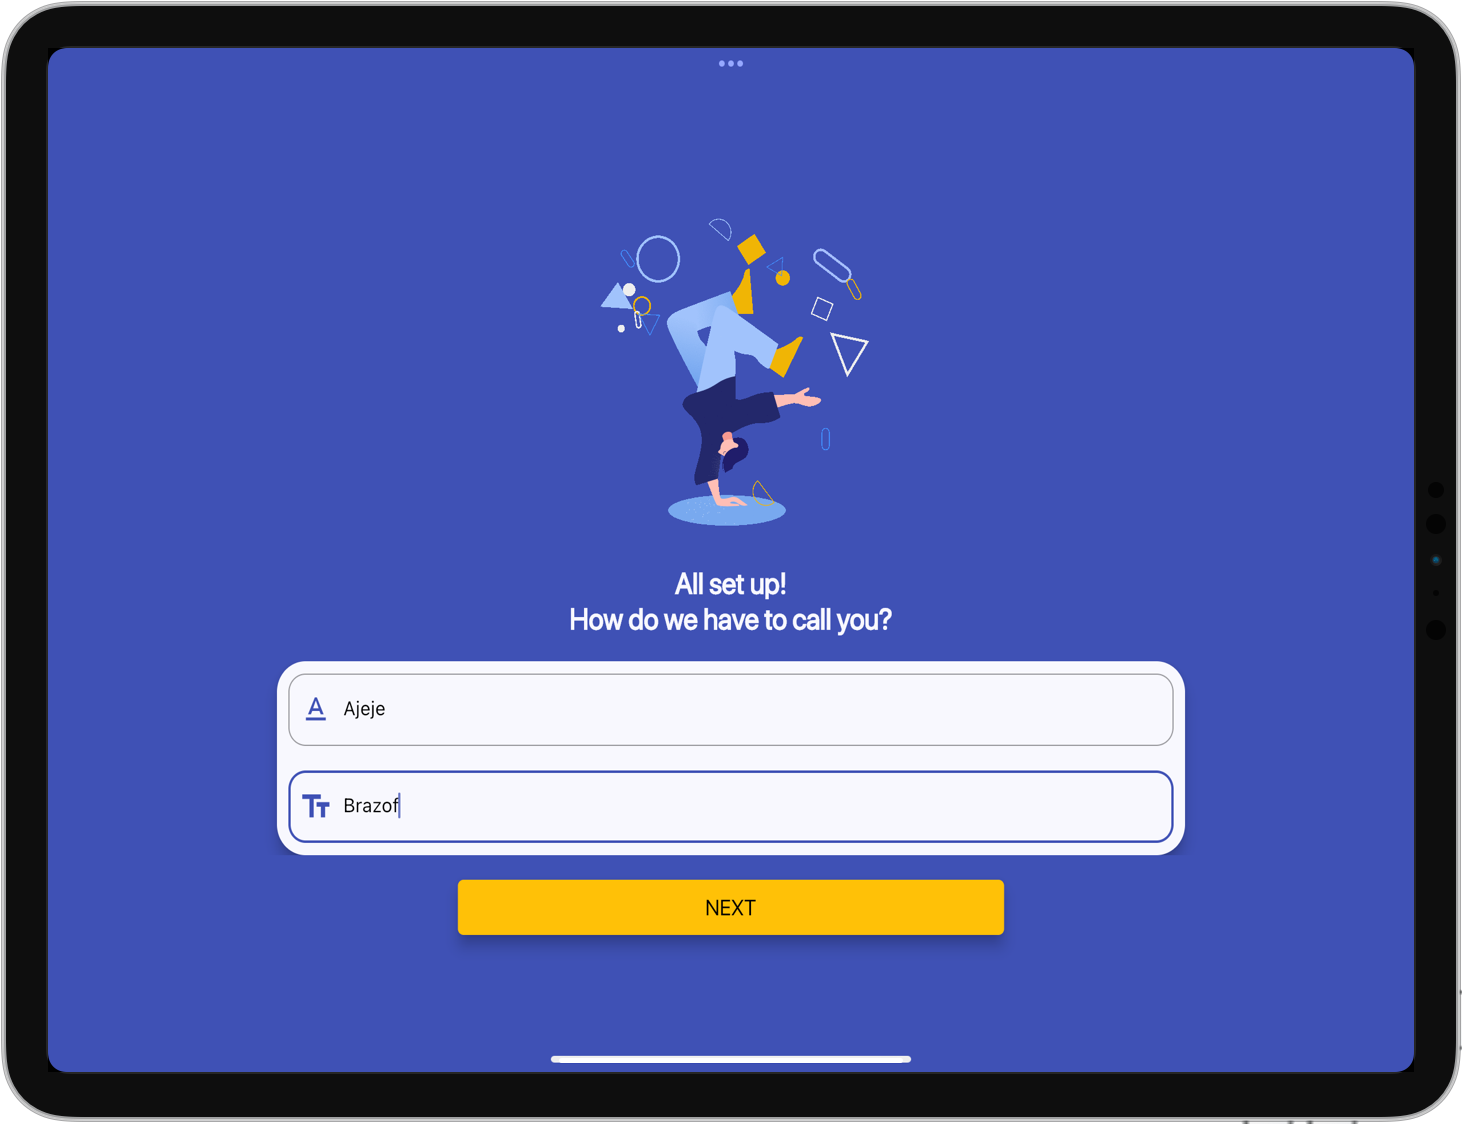
\includegraphics[scale=0.22]{./Images//Tablet_mocks/sign_up3_mod.png}
    \vspace*{-0.3cm}
    \caption{Tablet set display name page}
\end{figure}


\newgeometry{top=2cm}
\subsection{Home screen}
The homepage is designed to display all the products of a user (if he/she has any), or the products also from other family members if he/she belongs to a family group.
The screen also displays some useful information about the product, for example the expiration date.
There is also the possibility to add new products, by pressing the "+" button, adding them by using barcode or by simply adding them by name.
In addition, by pressing on a product, present in the product list, there is the possibility to view detailed information about that product, such as nutritional values, ingredients, etc.


\vspace*{1cm}
\begin{figure}[H]
  \begin{minipage}{0.5\textwidth}
  \centering
    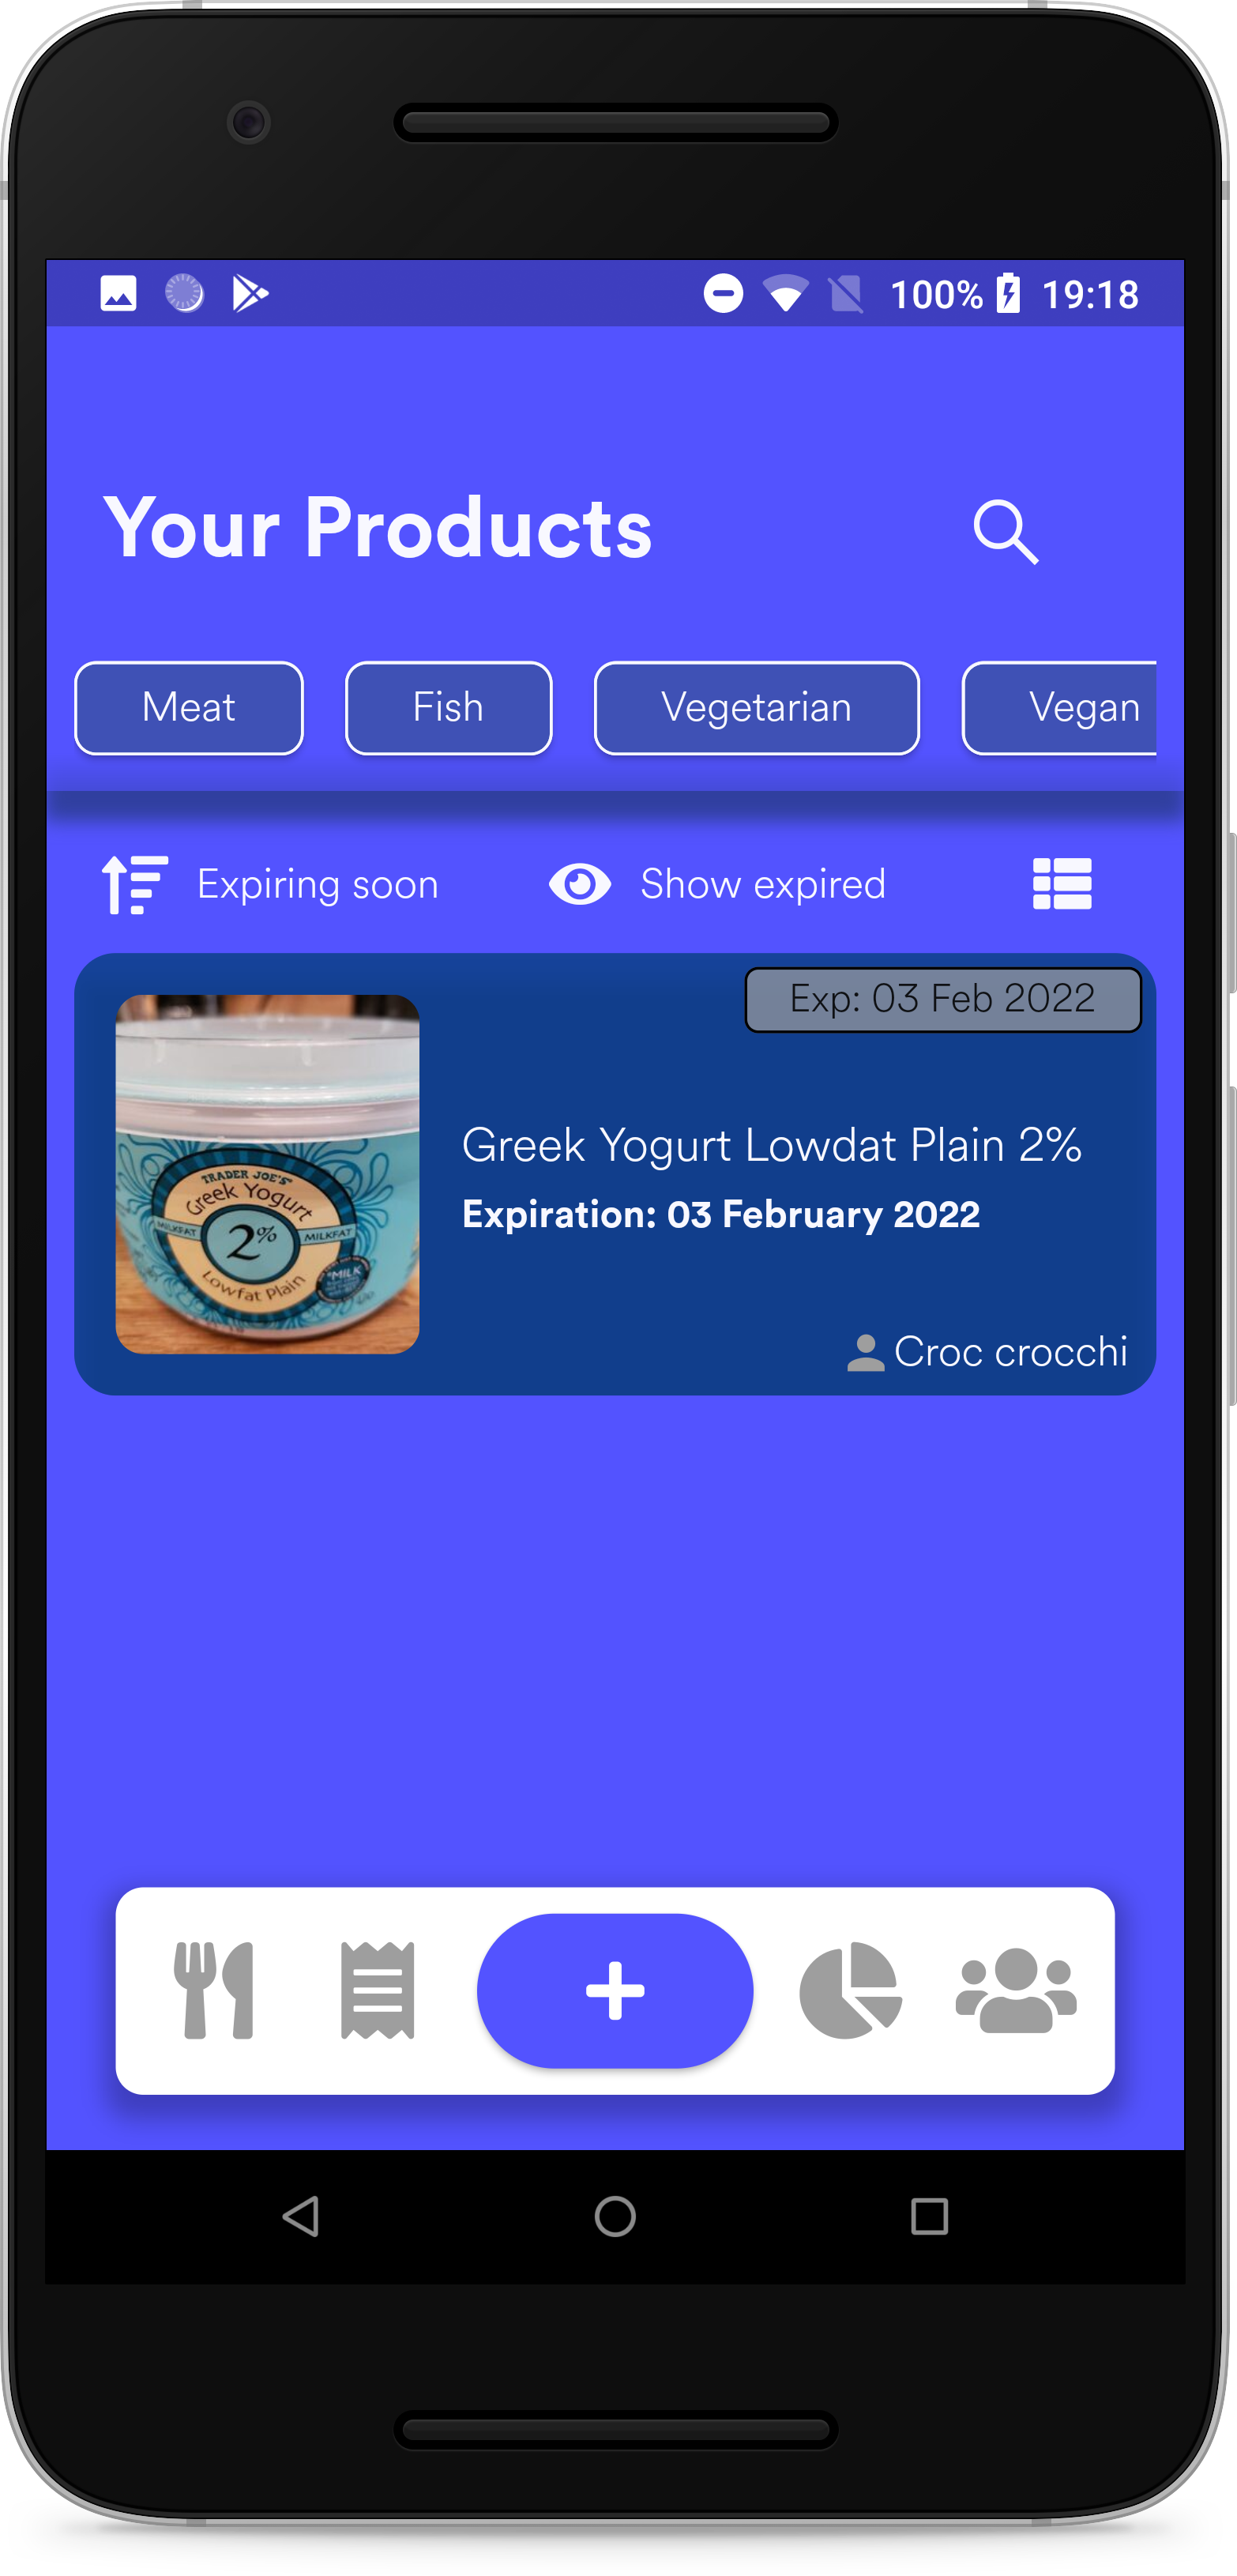
\includegraphics[width=38mm,scale=0.9]{./Images//Mobile_mocks/home1.png}
    \vspace*{-0.3cm}
    \caption{Mobile product list screen}
    \end{minipage}
\hfill
   \begin{minipage}{0.5\textwidth}
     \centering
     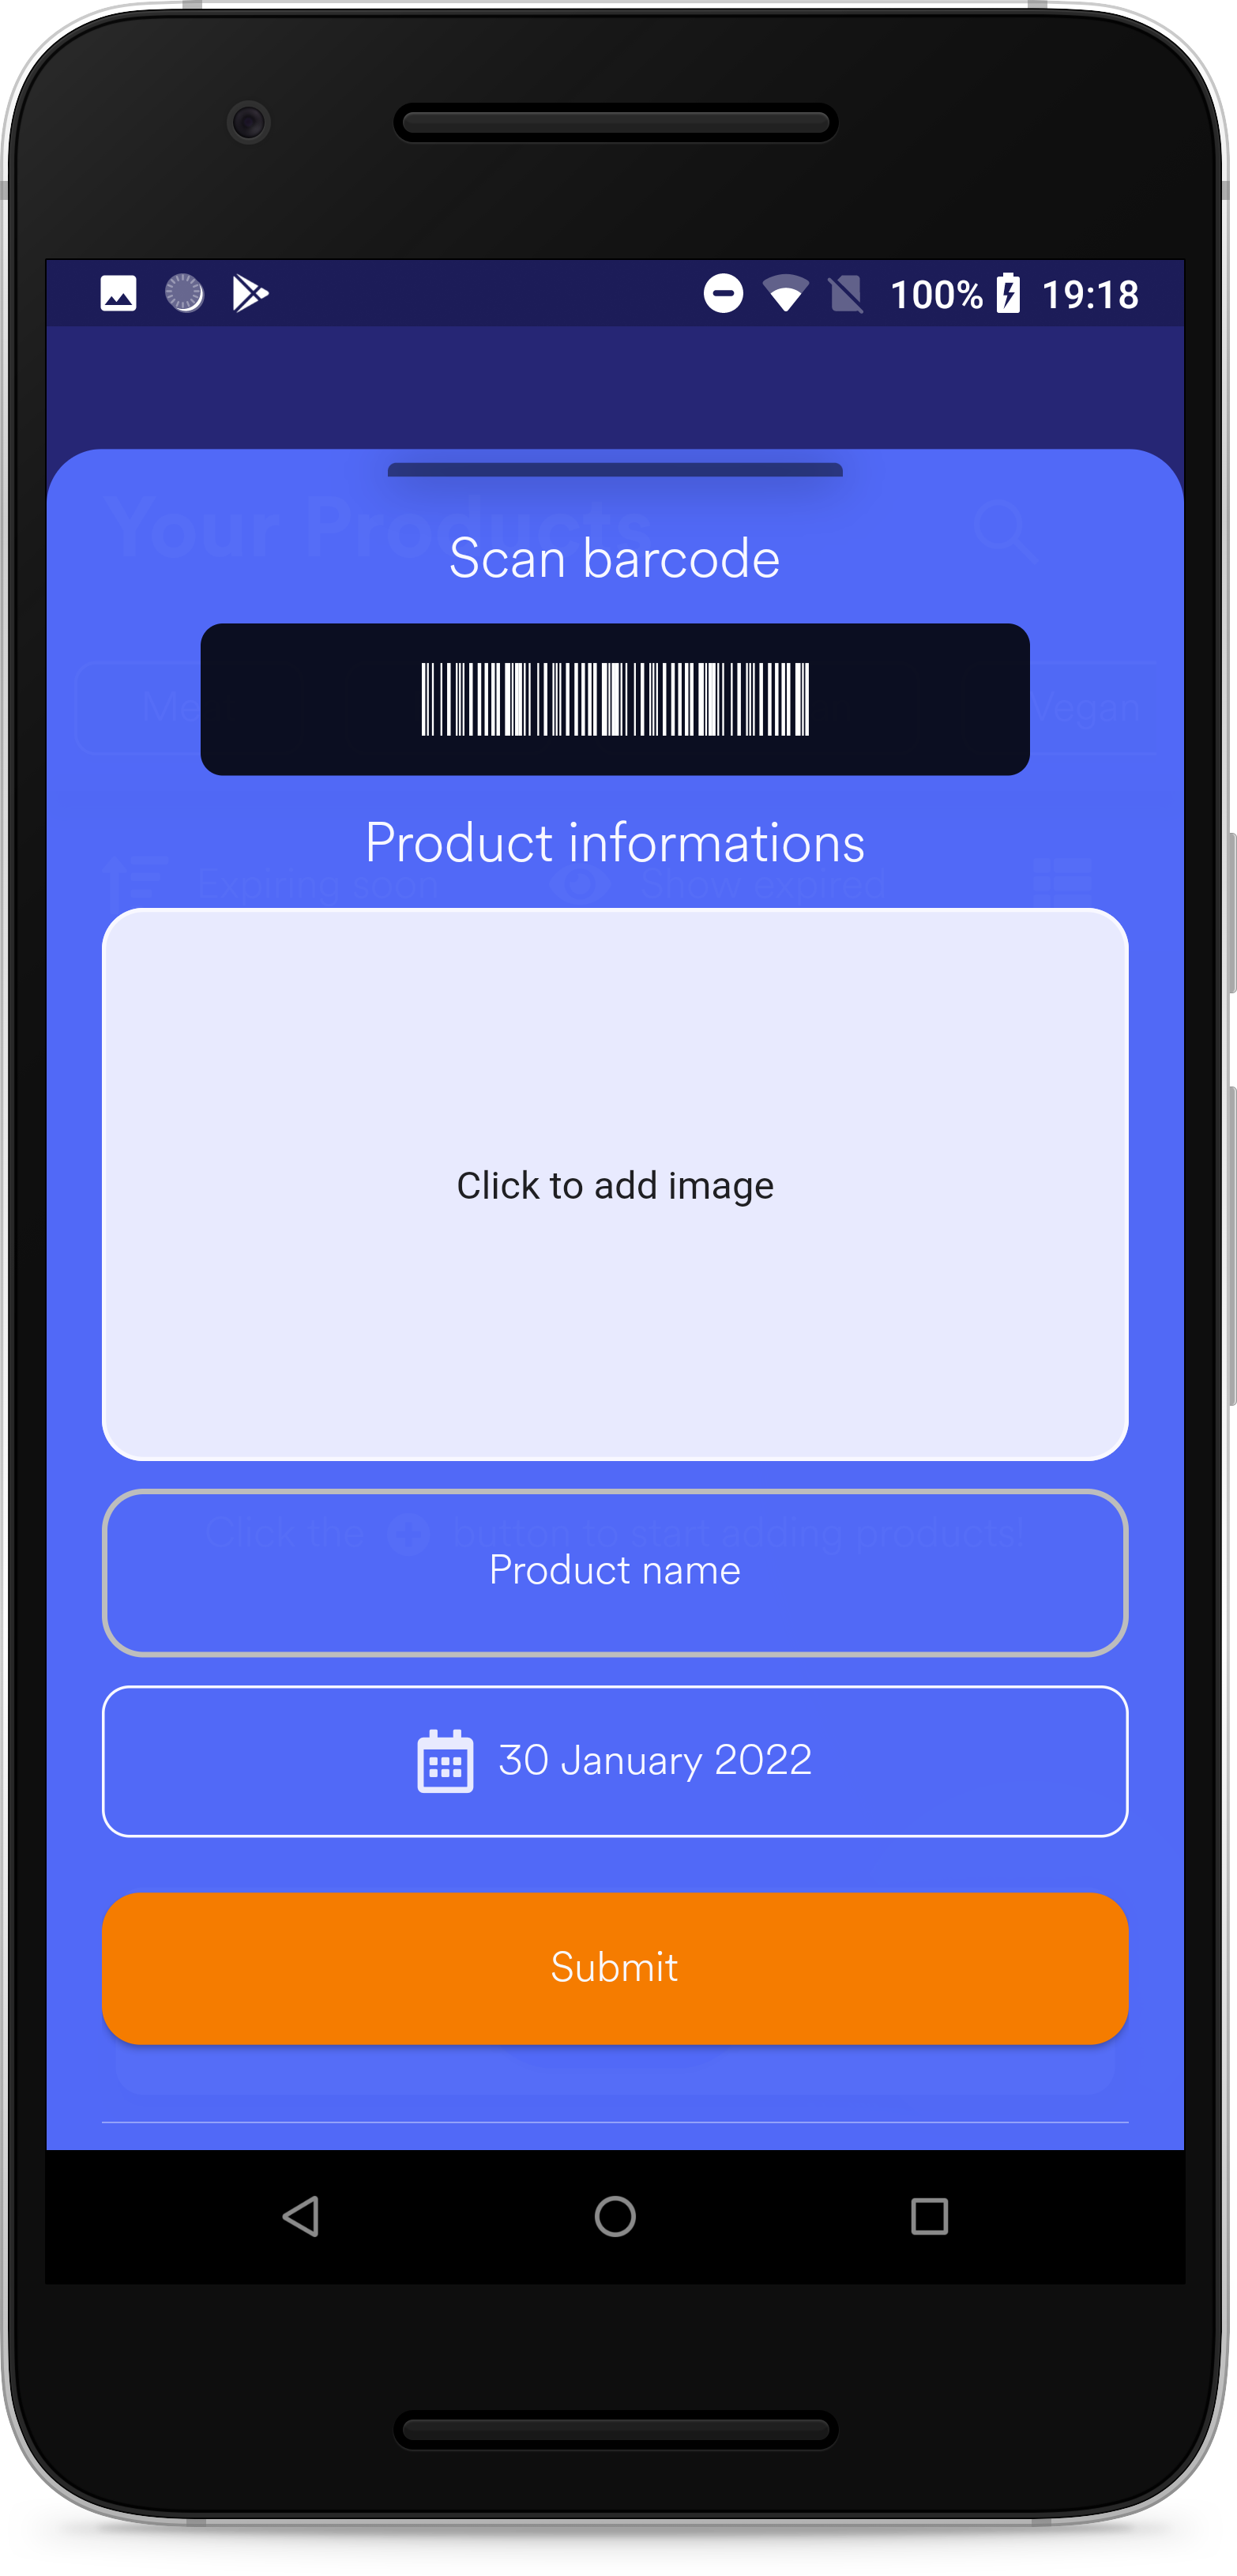
\includegraphics[width=38mm,scale=0.9]{./Images//Mobile_mocks/home2.png}
     \vspace*{-0.3cm}
     \caption{Mobile add product screen}
   \end{minipage}
\end{figure}

\vspace*{-0.3cm}
\begin{figure}[H]
  \centering
    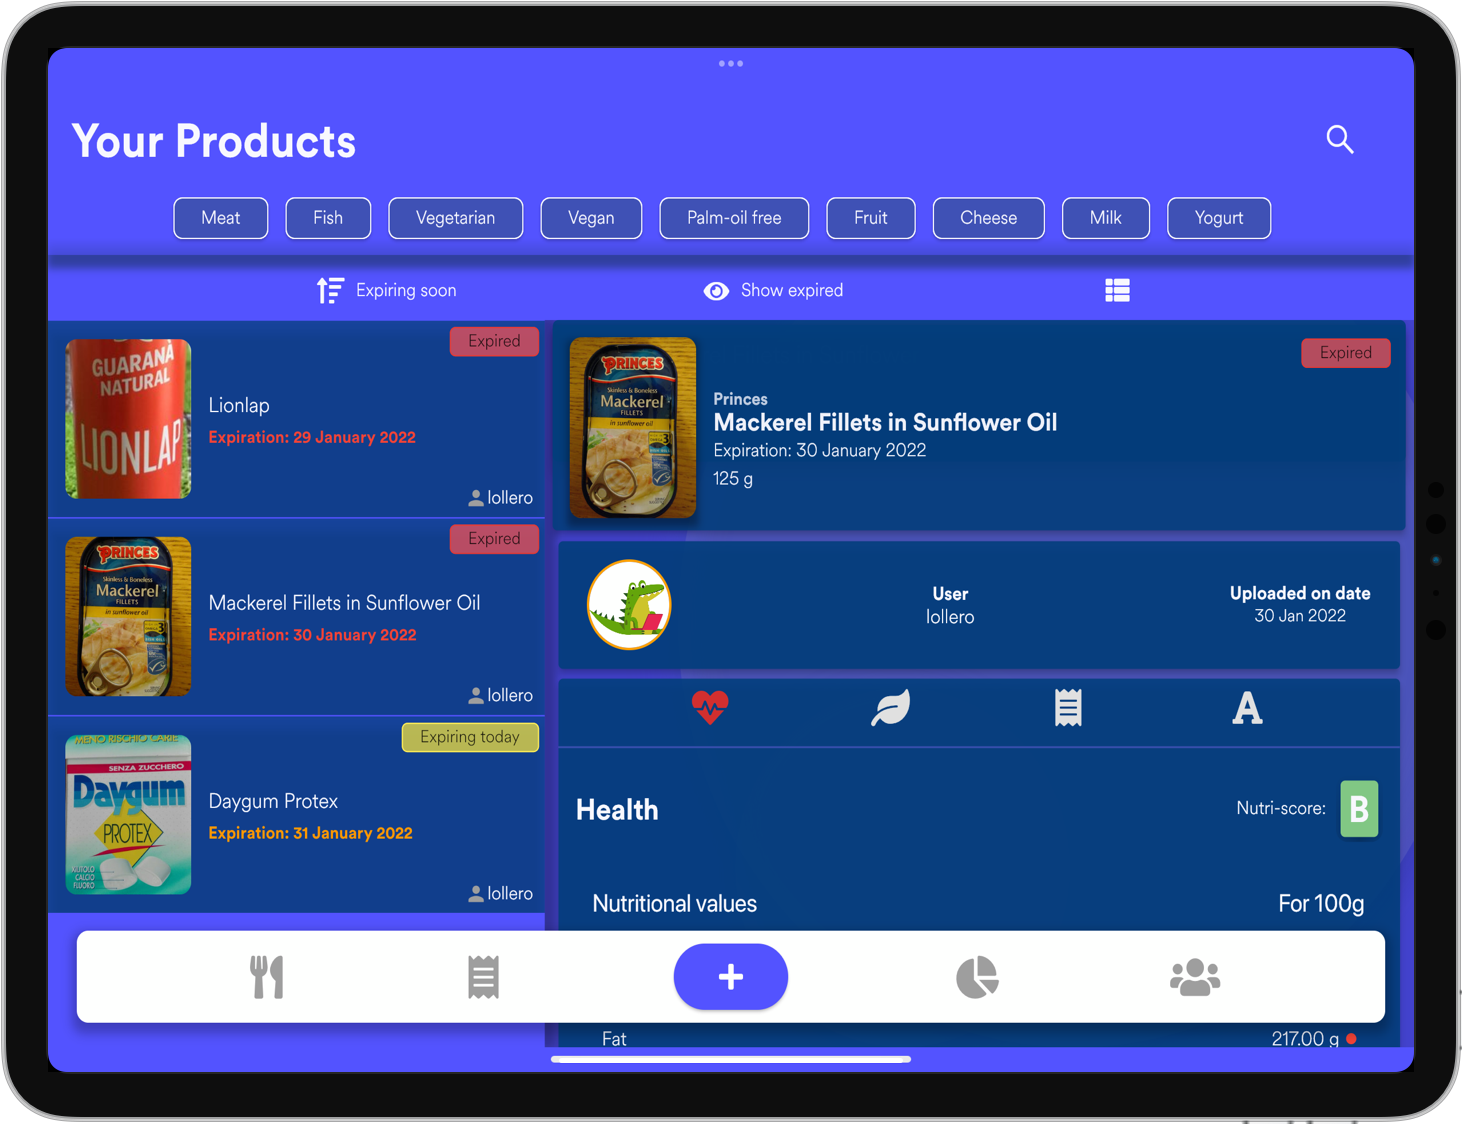
\includegraphics[scale=0.22]{./Images//Tablet_mocks/home1.png}
    \vspace*{-0.3cm}
    \caption{Tablet display product and details screen}
\end{figure}

\begin{figure}[H]
  \centering
    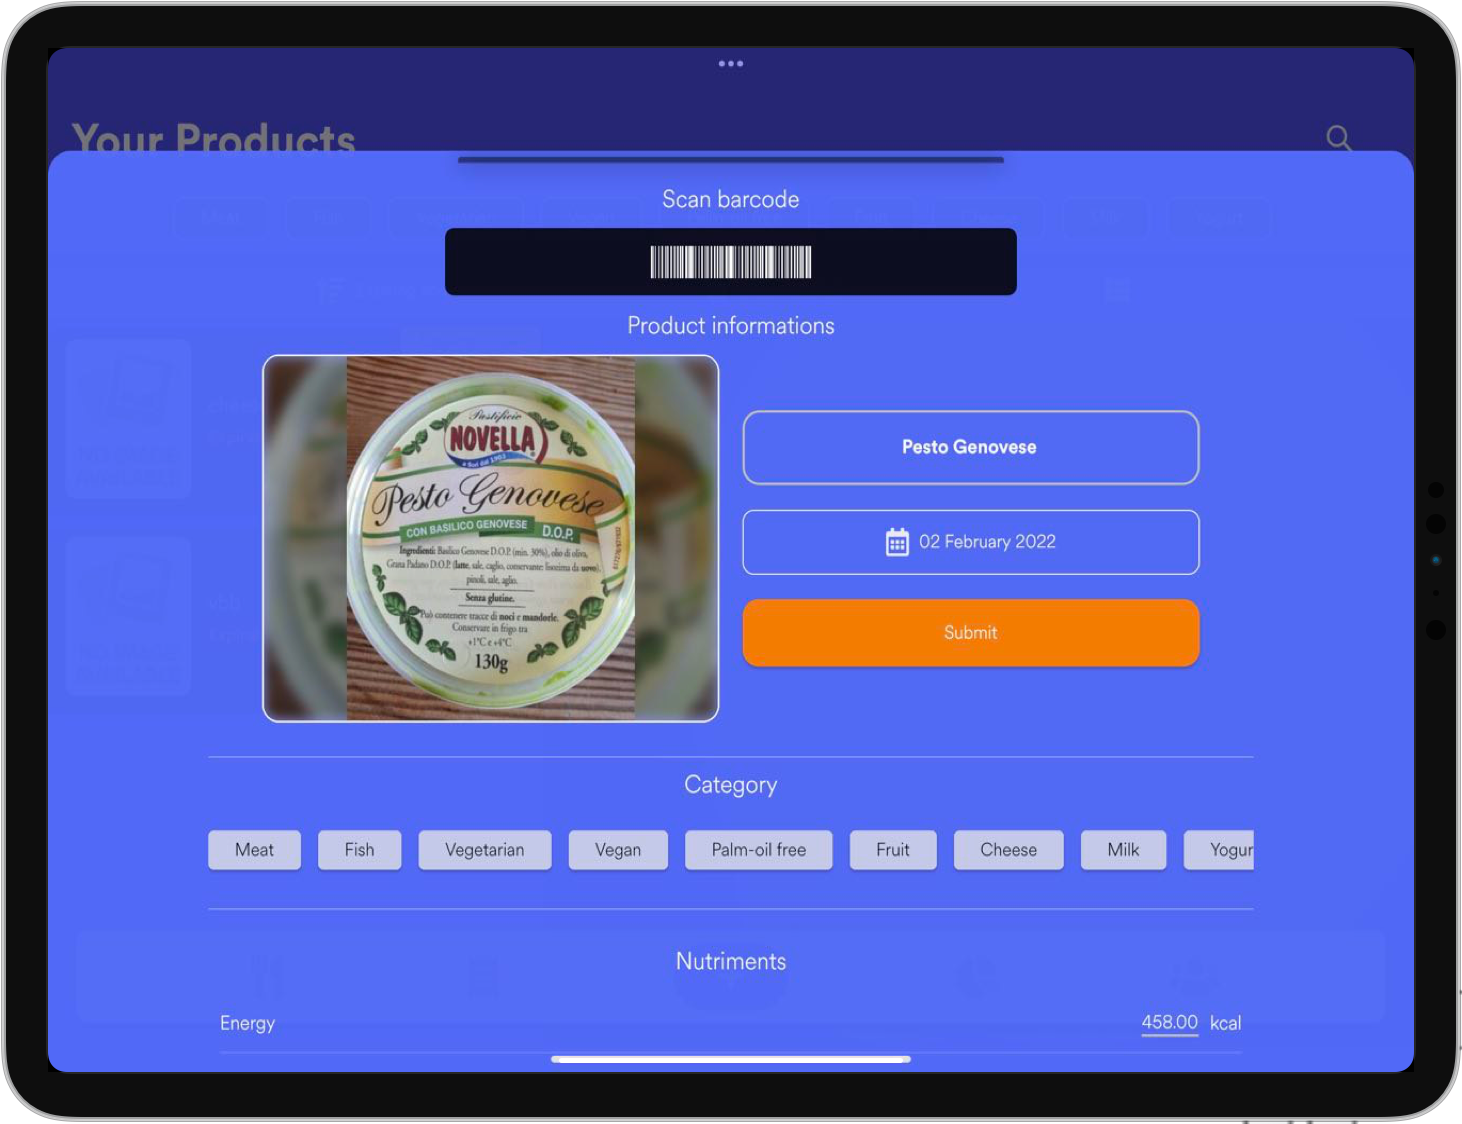
\includegraphics[scale=0.22]{./Images//Tablet_mocks/ipad_modal.png}
    \vspace*{-0.3cm}
    \caption{Add product view from ipad landscape}
\end{figure}
\restoregeometry


\subsection{Recipe Screen}
This section shows a list of recipes based on the products that users have.
By scrolling down the page, users can explore more and more recipes.
By tapping one of those recipes another screen is visualized, with the detail of the recipe: ingredients, preparation steps, preparing time, and servings.\newline

\vspace*{-0.3cm}
\begin{figure}[H]
  \begin{minipage}{0.5\textwidth}
  \centering
    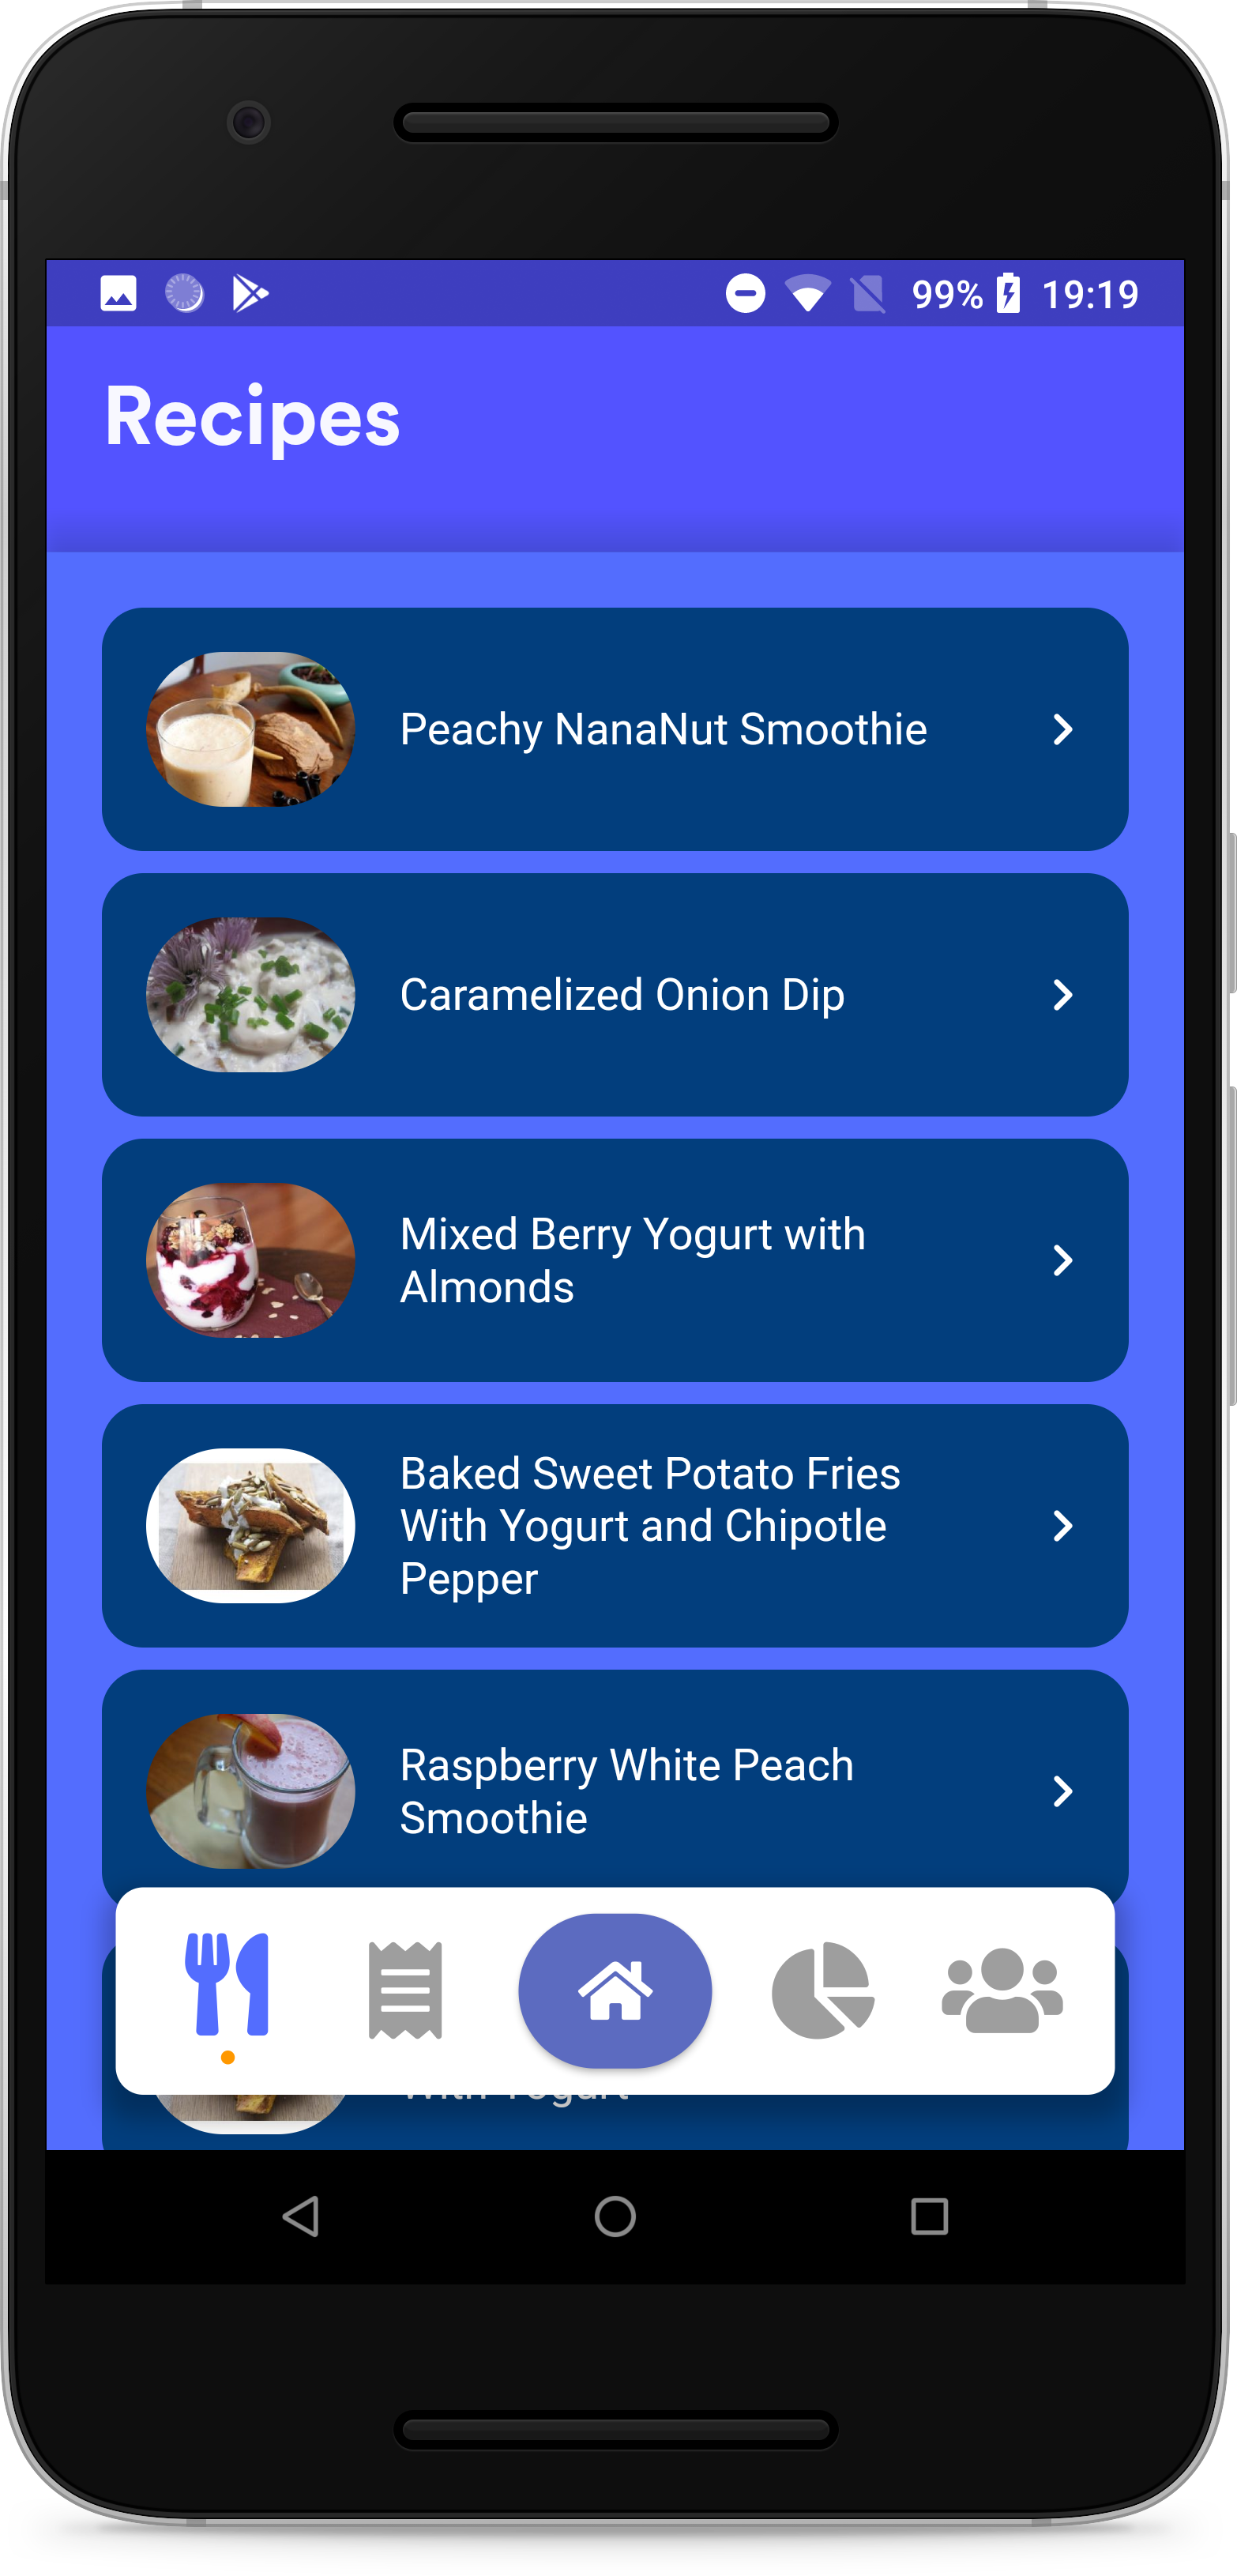
\includegraphics[width=42.mm,scale=0.9]{./Images//Mobile_mocks/recipe1.png}
    \vspace*{-0.3cm}
    \caption{Mobile recipe screen}
    \end{minipage}
\hfill
   \begin{minipage}{0.5\textwidth}
     \centering
     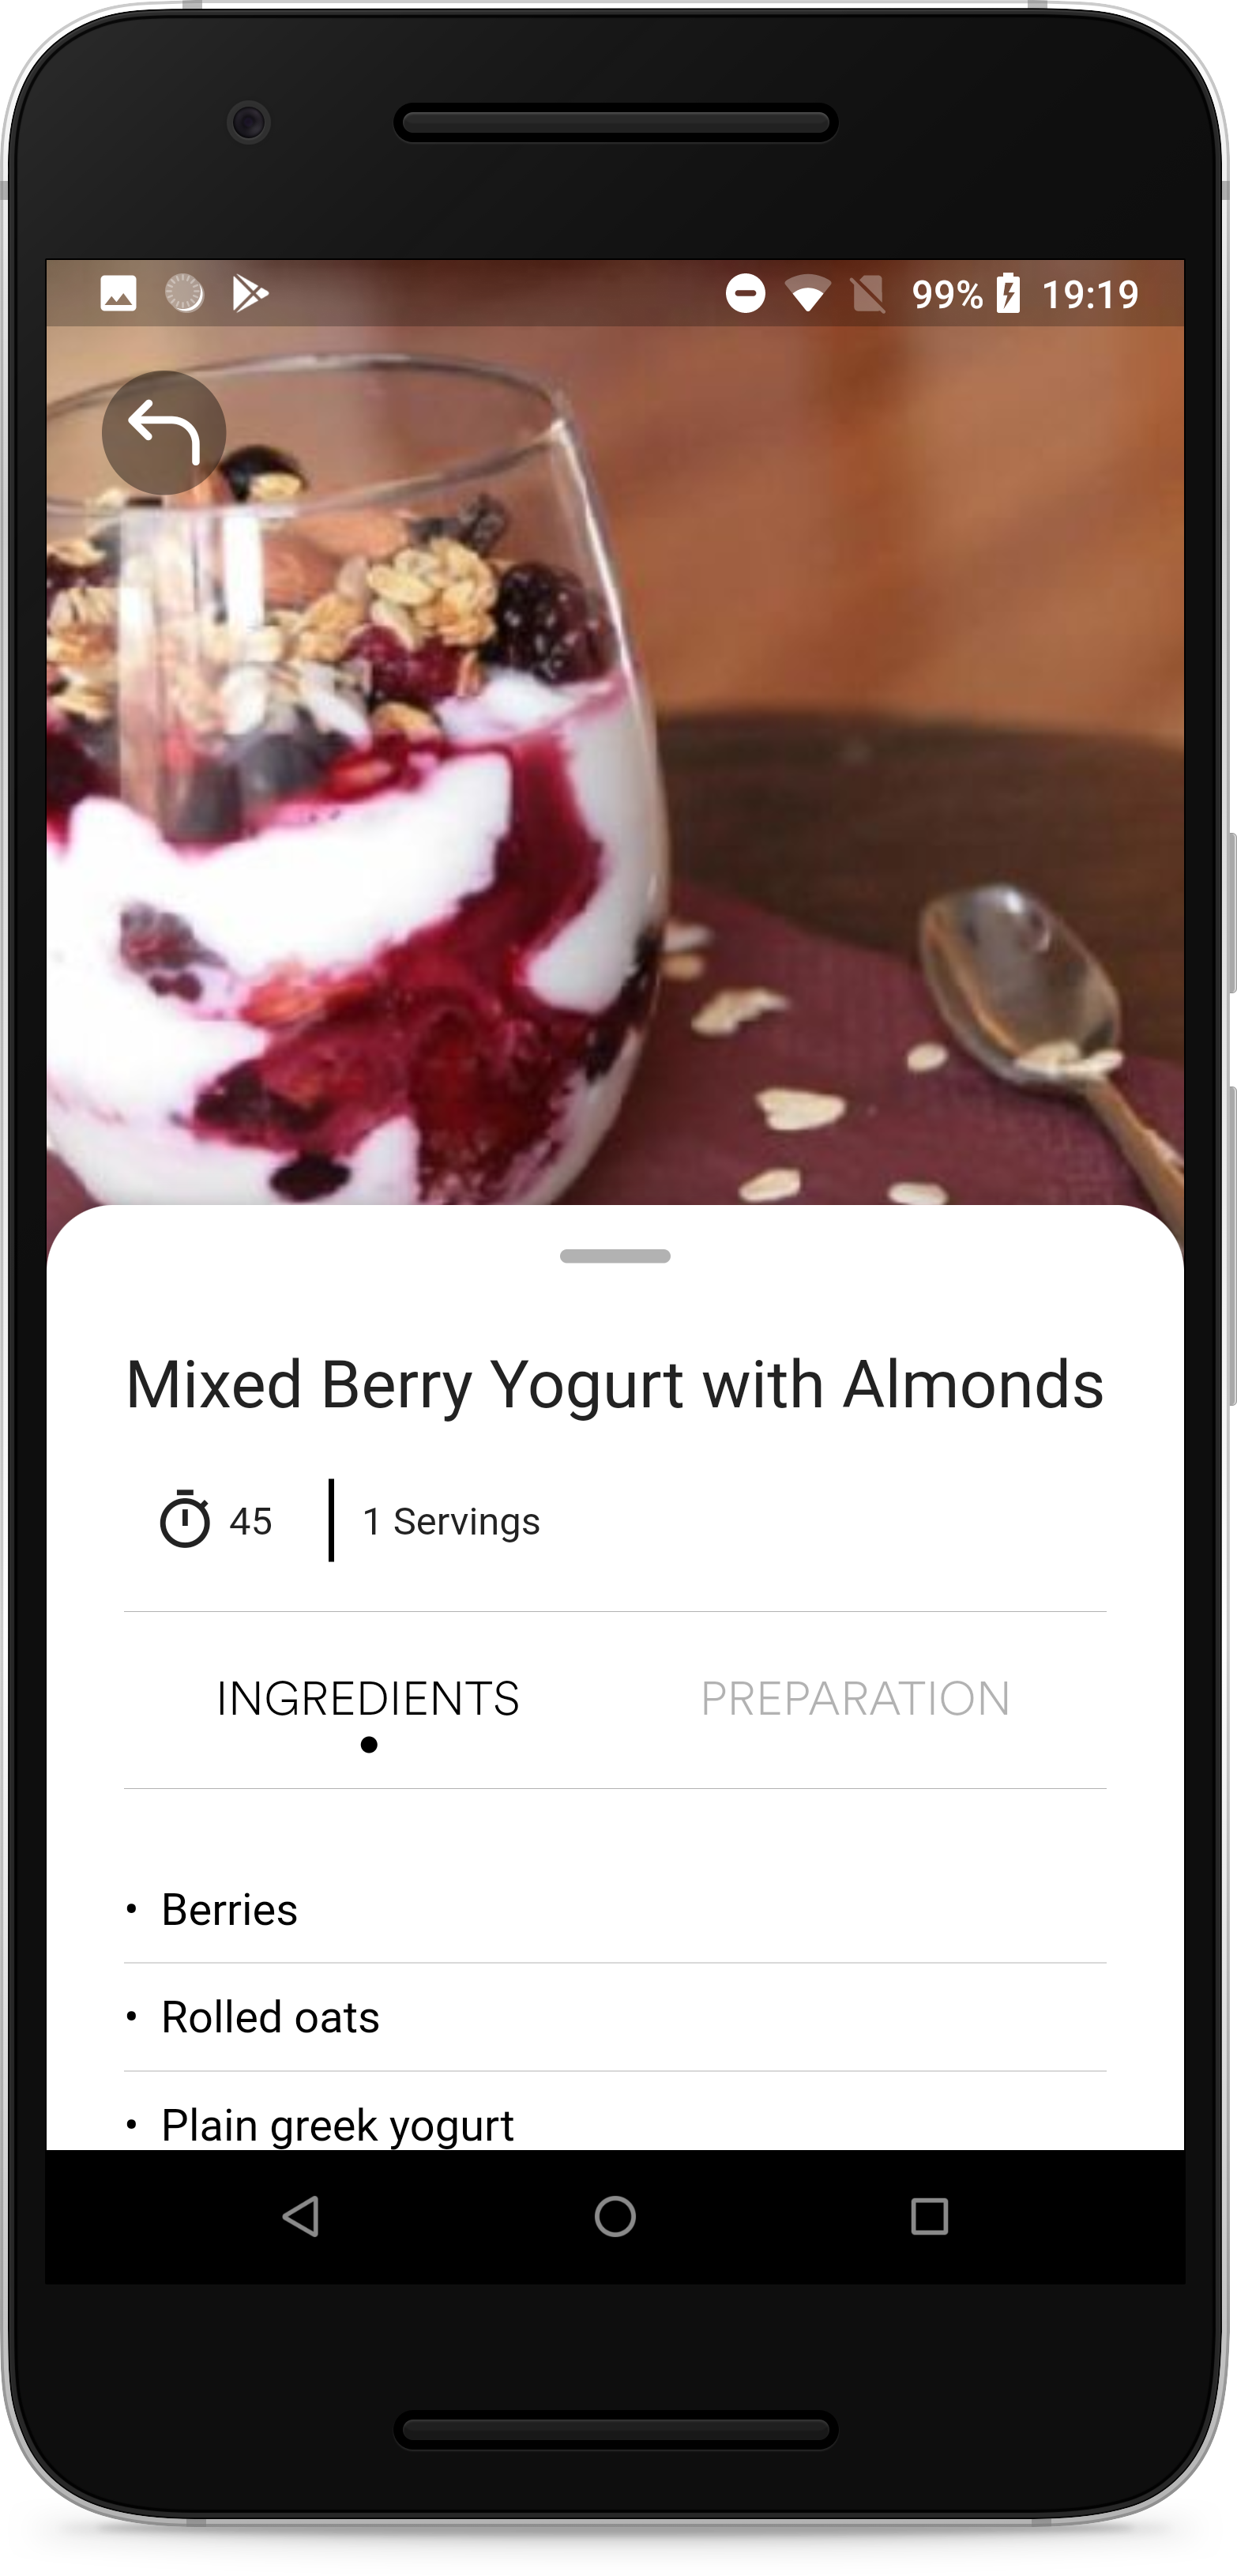
\includegraphics[width=42mm,scale=0.9]{./Images//Mobile_mocks/recipe2.png}
     \vspace*{-0.3cm}
     \caption{Mobile recipe detail screen}
   \end{minipage}
\end{figure}
\subsection{Shopping Lists Screen}
The shopping lists screen manage, as the name suggests, the possibility to create lists with products.
Those lists are useful when a user goes for grocery, and they're helpful to remind about products to buy.
In top right part of the screen, there's a button named "Add List +", once tapped create a new list, where users can add products.\newline

\begin{figure}[H]
  \centering
    \vspace*{-0.3cm}
     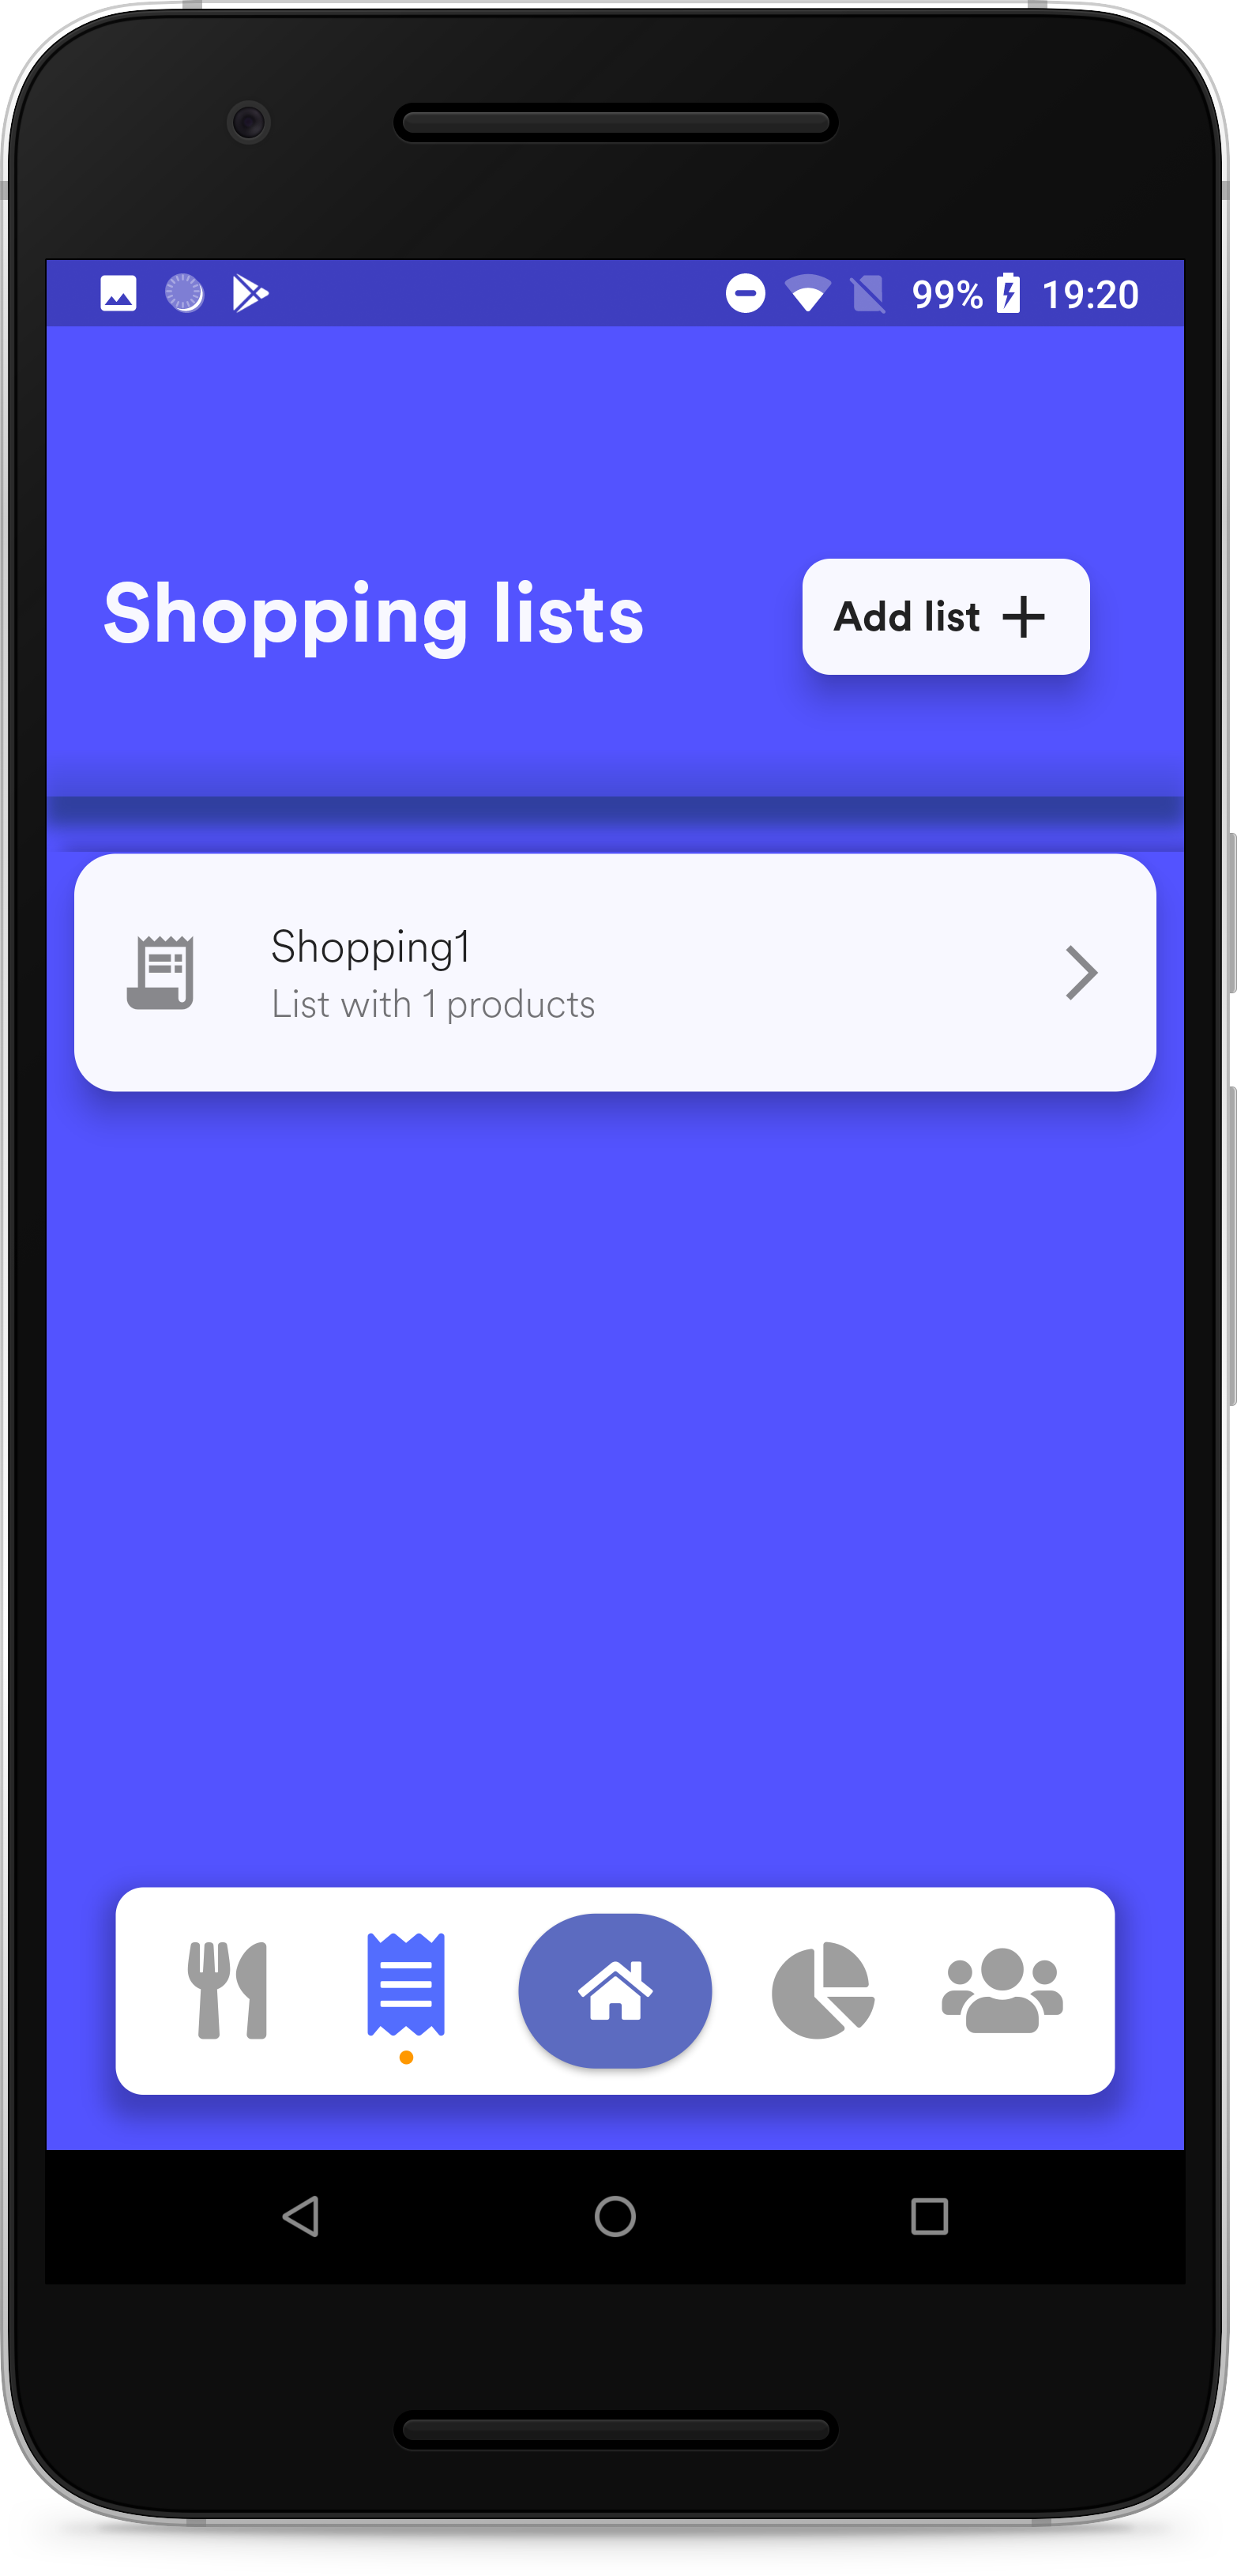
\includegraphics[width=42mm,scale=0.9]{./Images//Mobile_mocks/shopping1.png}
     \vspace*{-0.3cm}
     \caption{Mobile shopping list screen}
\end{figure}

\vspace*{-0.3cm}
\begin{figure}[H]
  \centering
    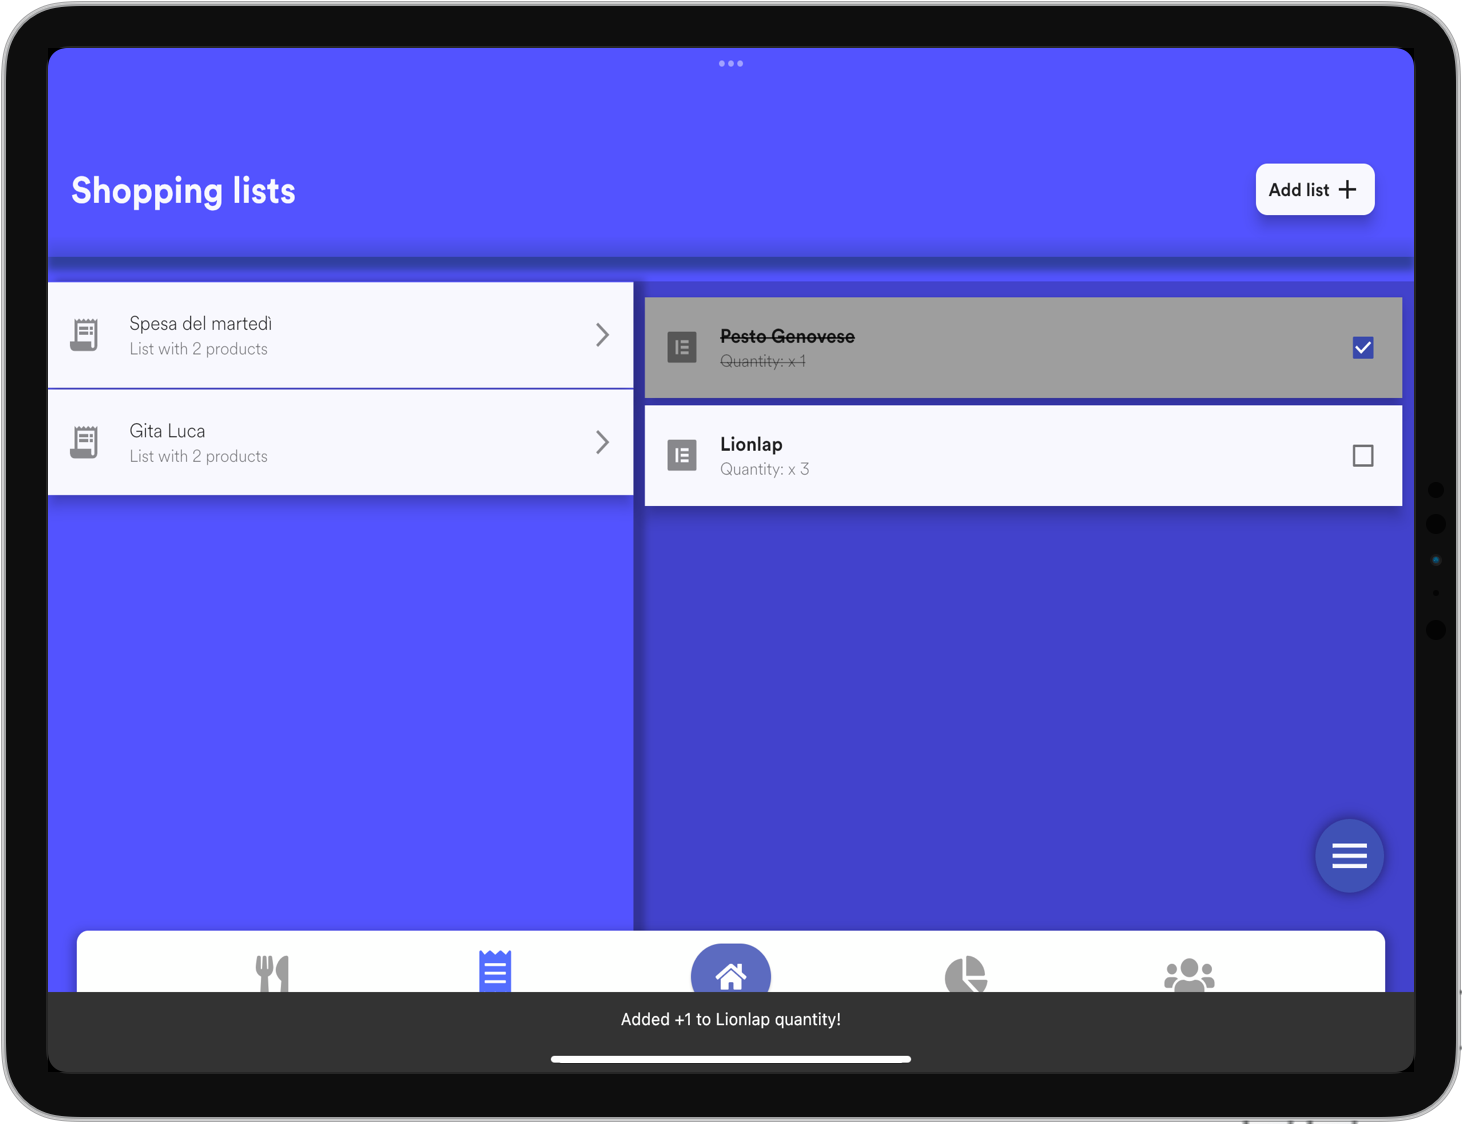
\includegraphics[scale=0.22]{./Images//Tablet_mocks/shopping1.png}
    \vspace*{-0.3cm}
    \caption{Tablet shopping list screen}
\end{figure}
\newgeometry{top=2cm}
\subsection{Statistics Screen}
This screen displays statistical data regarding products nutritional values.
In particular there are 4 donut charts, representing the overall quantity of sugar, fat, saturated-fat and salt in the products.
Every chart represents, for each value, three scores: "High", "Moderate" and "Low".

\begin{figure}[H]
  \centering
    \vspace*{-0.3cm}
     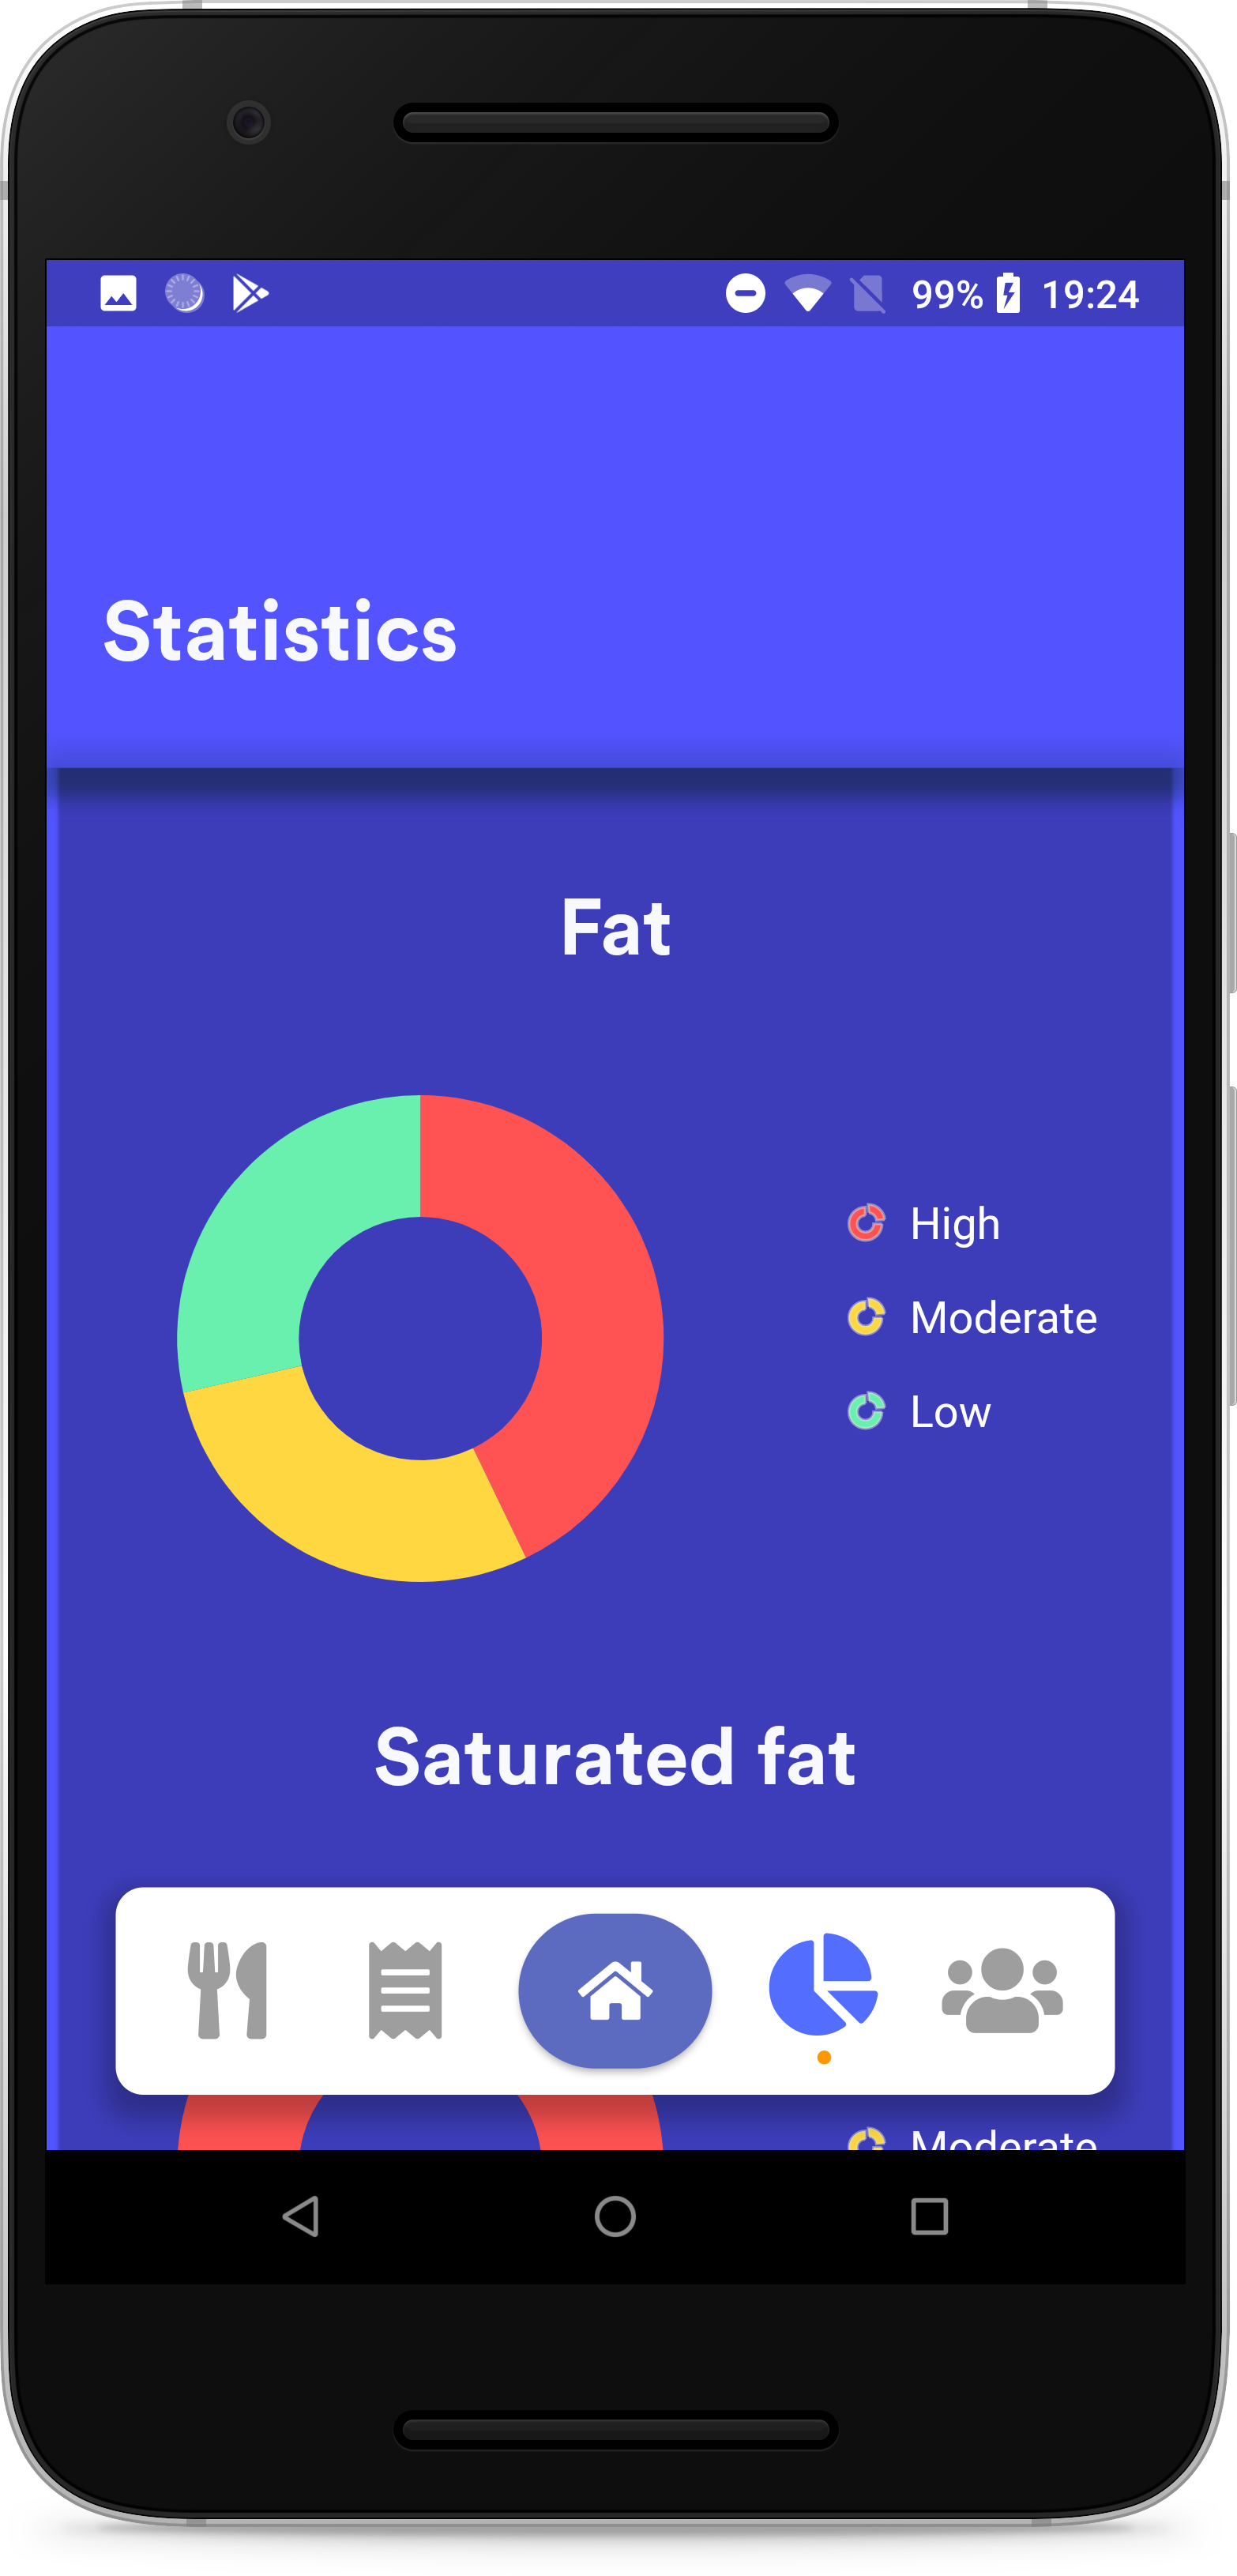
\includegraphics[width=42mm,scale=0.9]{./Images//Mobile_mocks/statistics1.png}
     \vspace*{-0.3cm}
     \caption{Mobile statistics screen}
\end{figure}

\vspace*{-0.3cm}
\begin{figure}[H]
  \centering
    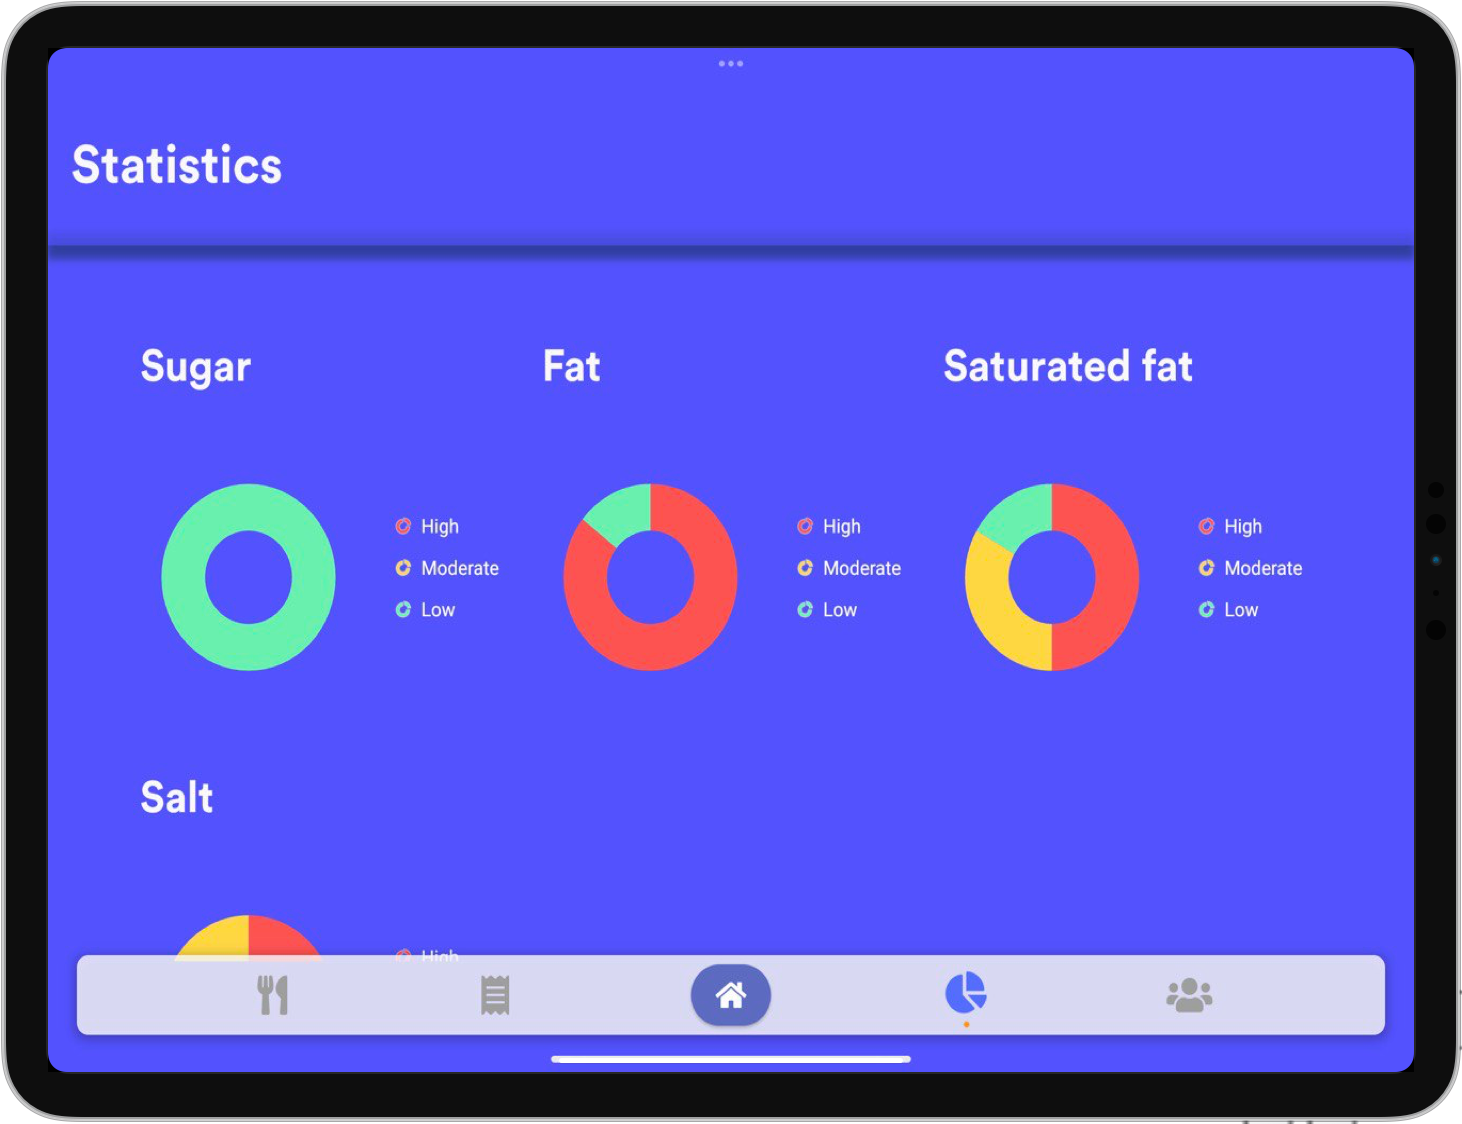
\includegraphics[scale=0.22]{./Images//Tablet_mocks/statistics1.png}
    \vspace*{-0.3cm}
    \caption{Tablet statistics screen}
\end{figure}
\subsection{User Info Screen}
The user info screen is the last that users can access through the tab selector. It shows the profile image of the user at the top, with his/her nickname and email. Below the screen is divided in two main subsections:
\begin{itemize}
    \item Account: it contains two buttons, "change name" and "delete account", that gives to the users the possibility to change their display name and delete their account.
    \item Family: this subsection manage the synchronization with family members, and contains 4 buttons: "share family" that give to the users the possibility to generate a qr code and give to the other users the possibility to join their family; "leave family", once pressed, pop up an alert dialogue to ask users if they really want to leave the family group (whether they're a part of it); "family members" open a new screen and shows the list of users of a family; "join family" pop up a dialog where users have the possibility to join a family group by scanning a qr code or inserting manually the id of a family group.
\end{itemize}

Finally at the bottom there are some other buttons and finally the log out button.\newpage

\vspace*{-0.3cm}
\begin{figure}[H]
  \begin{minipage}{0.5\textwidth}
  \centering
    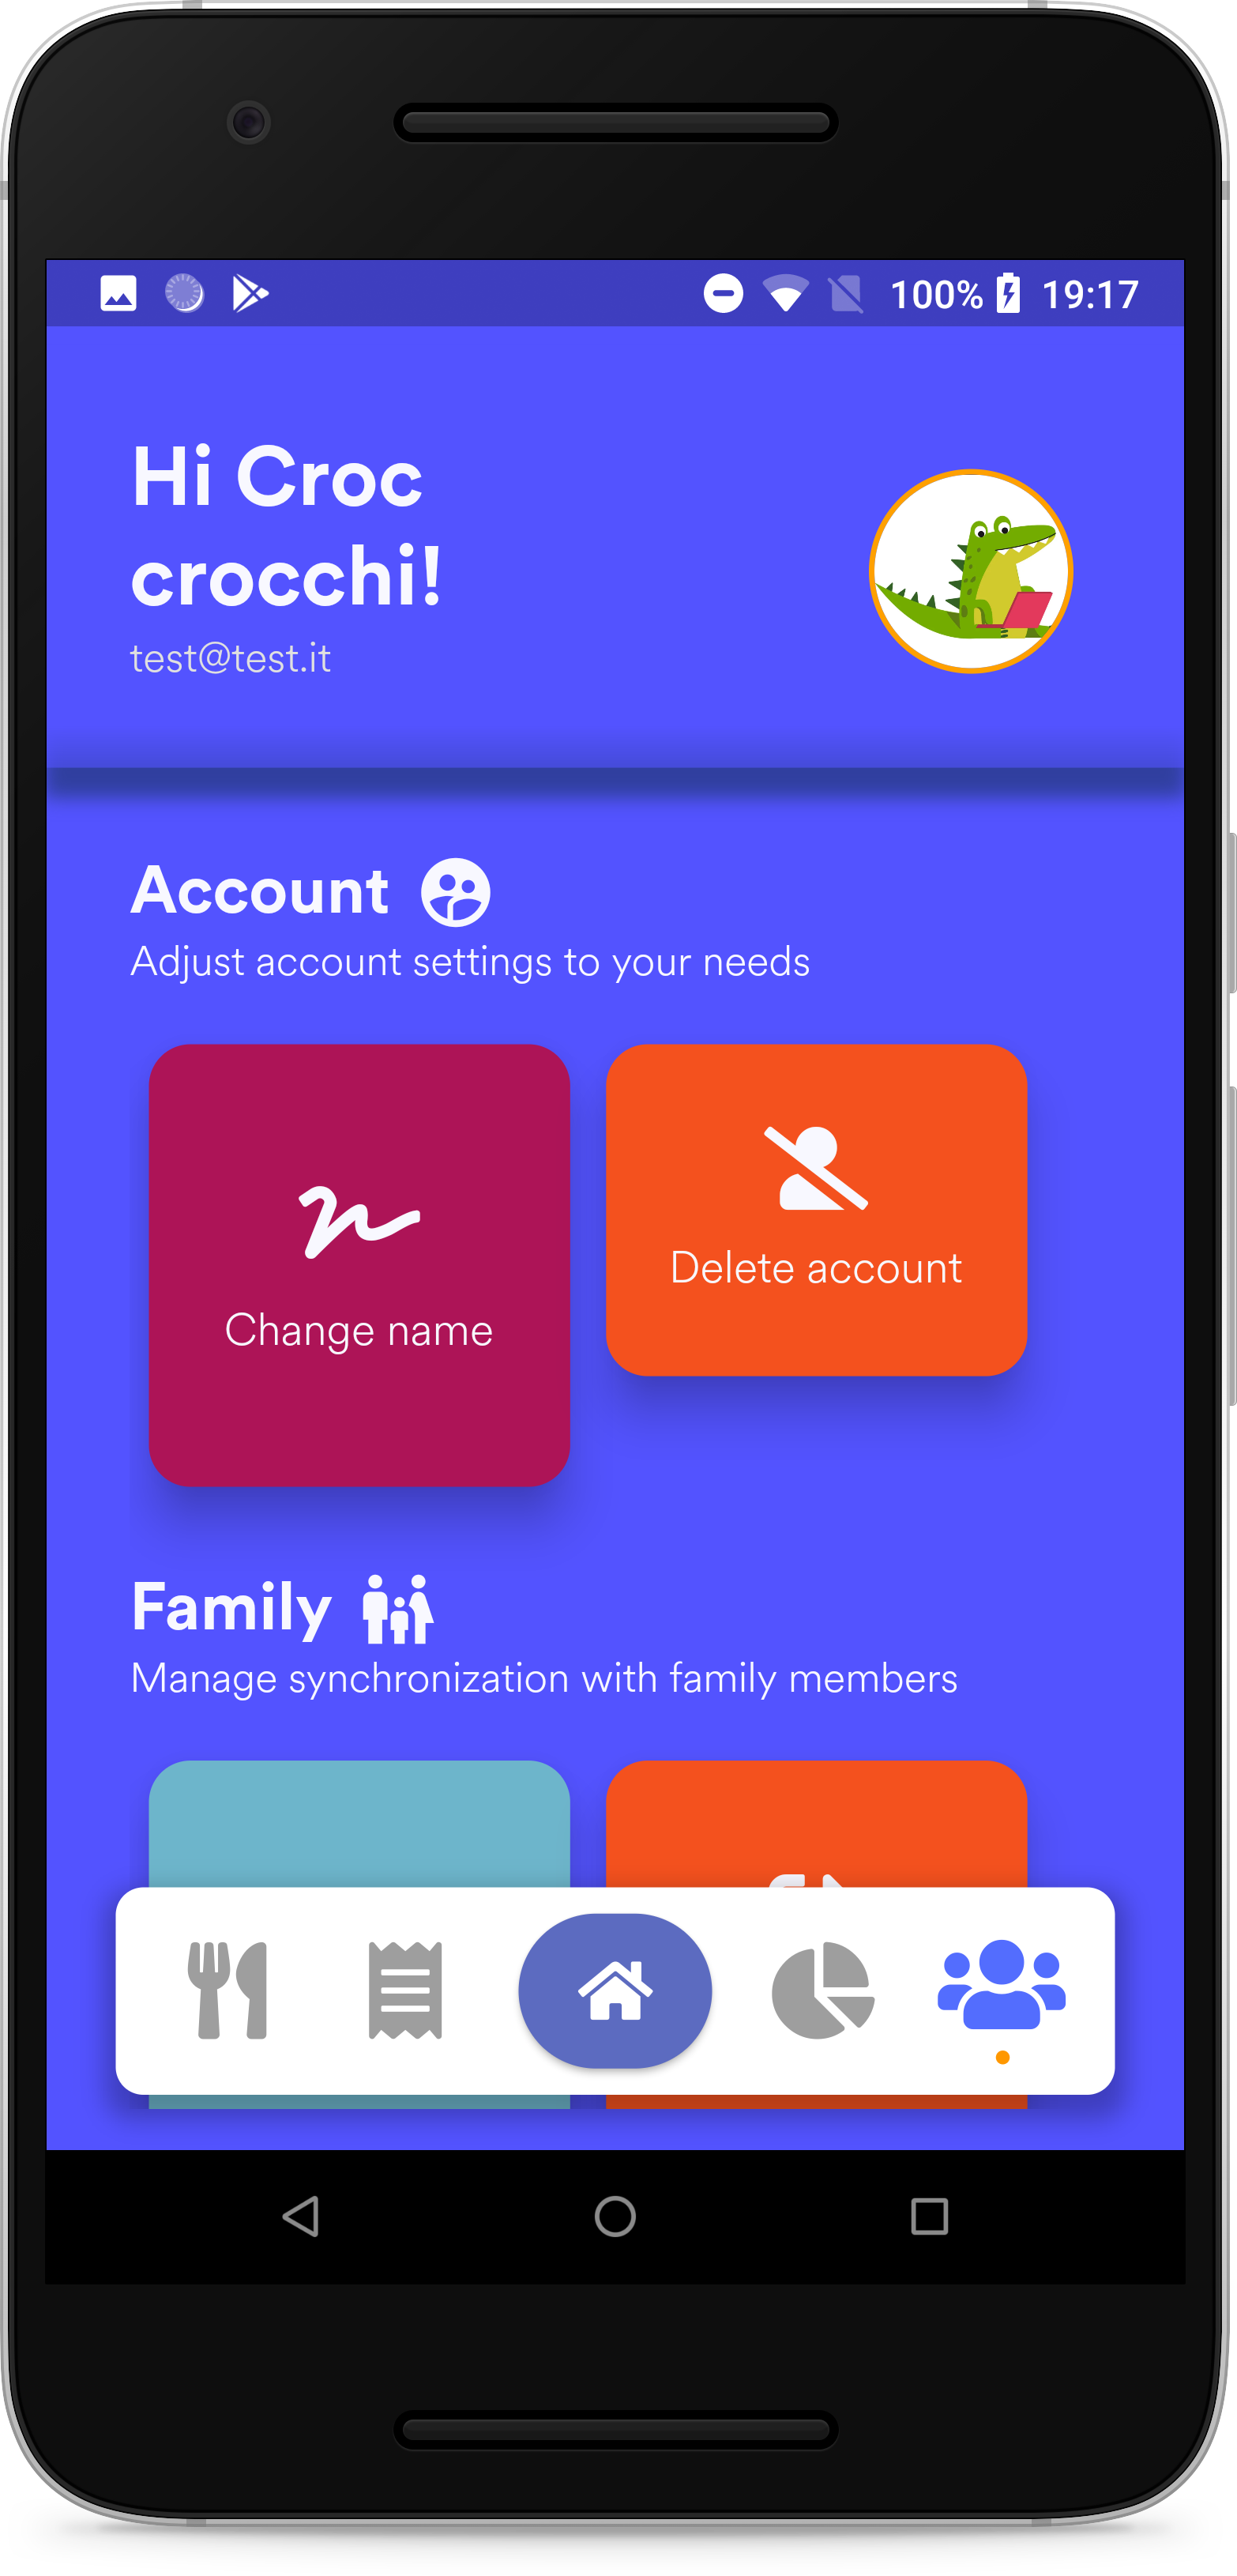
\includegraphics[width=42.mm,scale=0.9]{./Images//Mobile_mocks/user1.png}
    \vspace*{-0.3cm}
    \caption{Mobile user info screen 1}
    \end{minipage}
\hfill
   \begin{minipage}{0.5\textwidth}
     \centering
     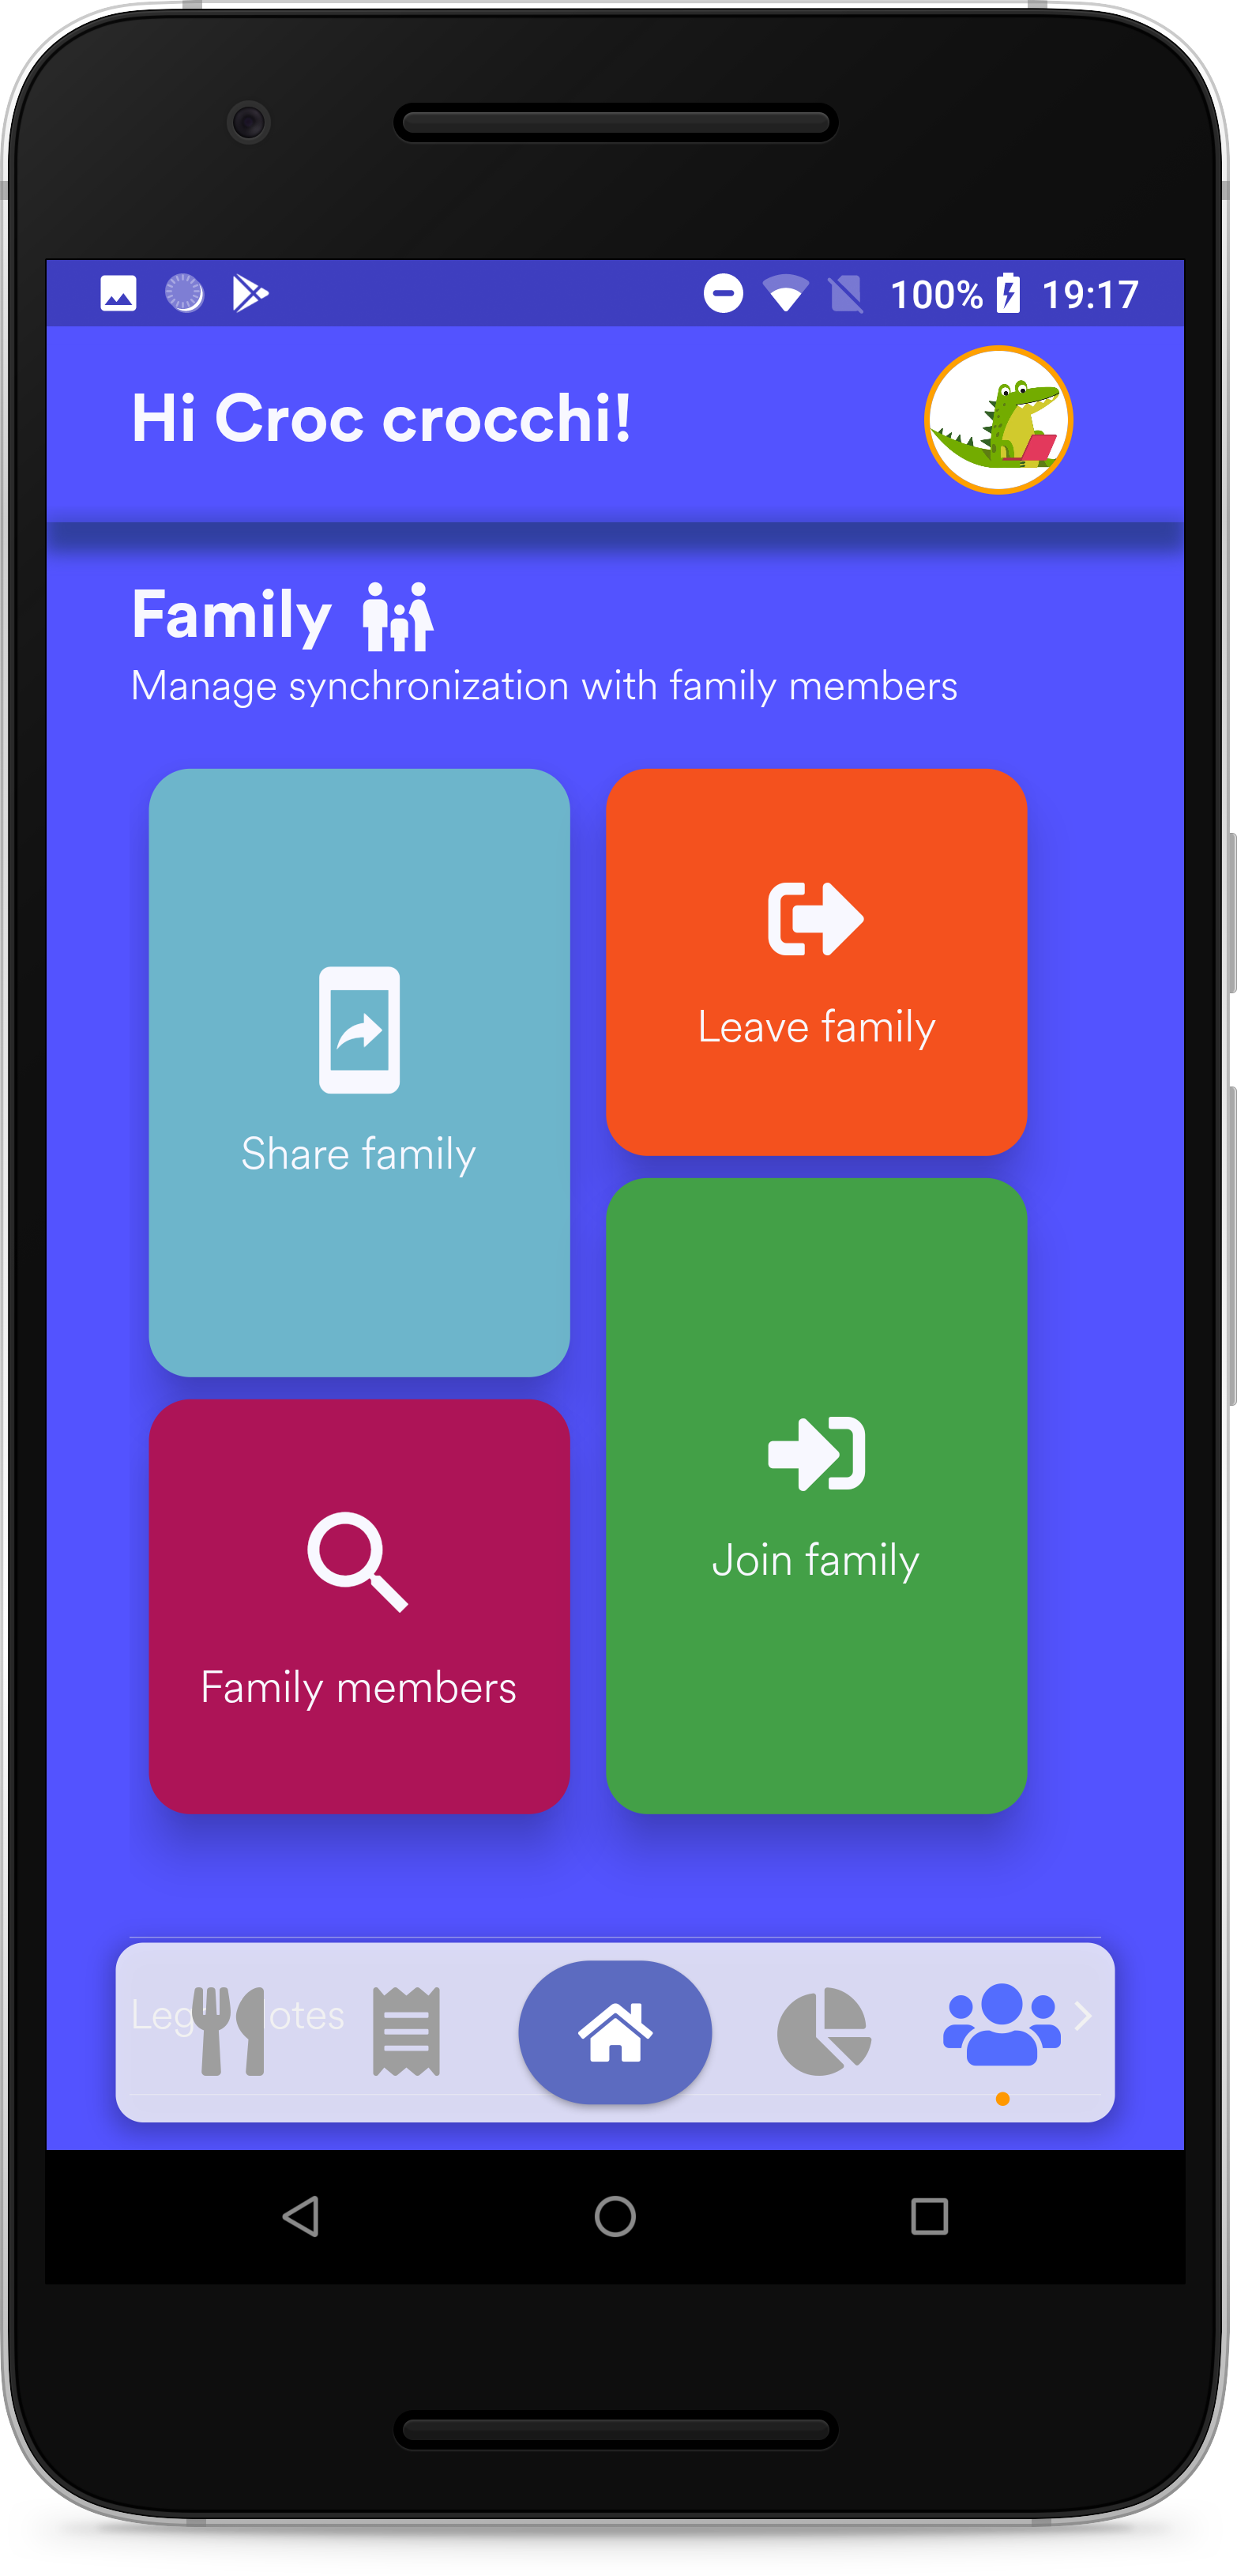
\includegraphics[width=42mm,scale=0.9]{./Images//Mobile_mocks/user2.png}
     \vspace*{-0.3cm}
     \caption{Mobile user info screen 2}
   \end{minipage}
\end{figure}

\vspace*{-0.3cm}
\begin{figure}[H]
  \centering
    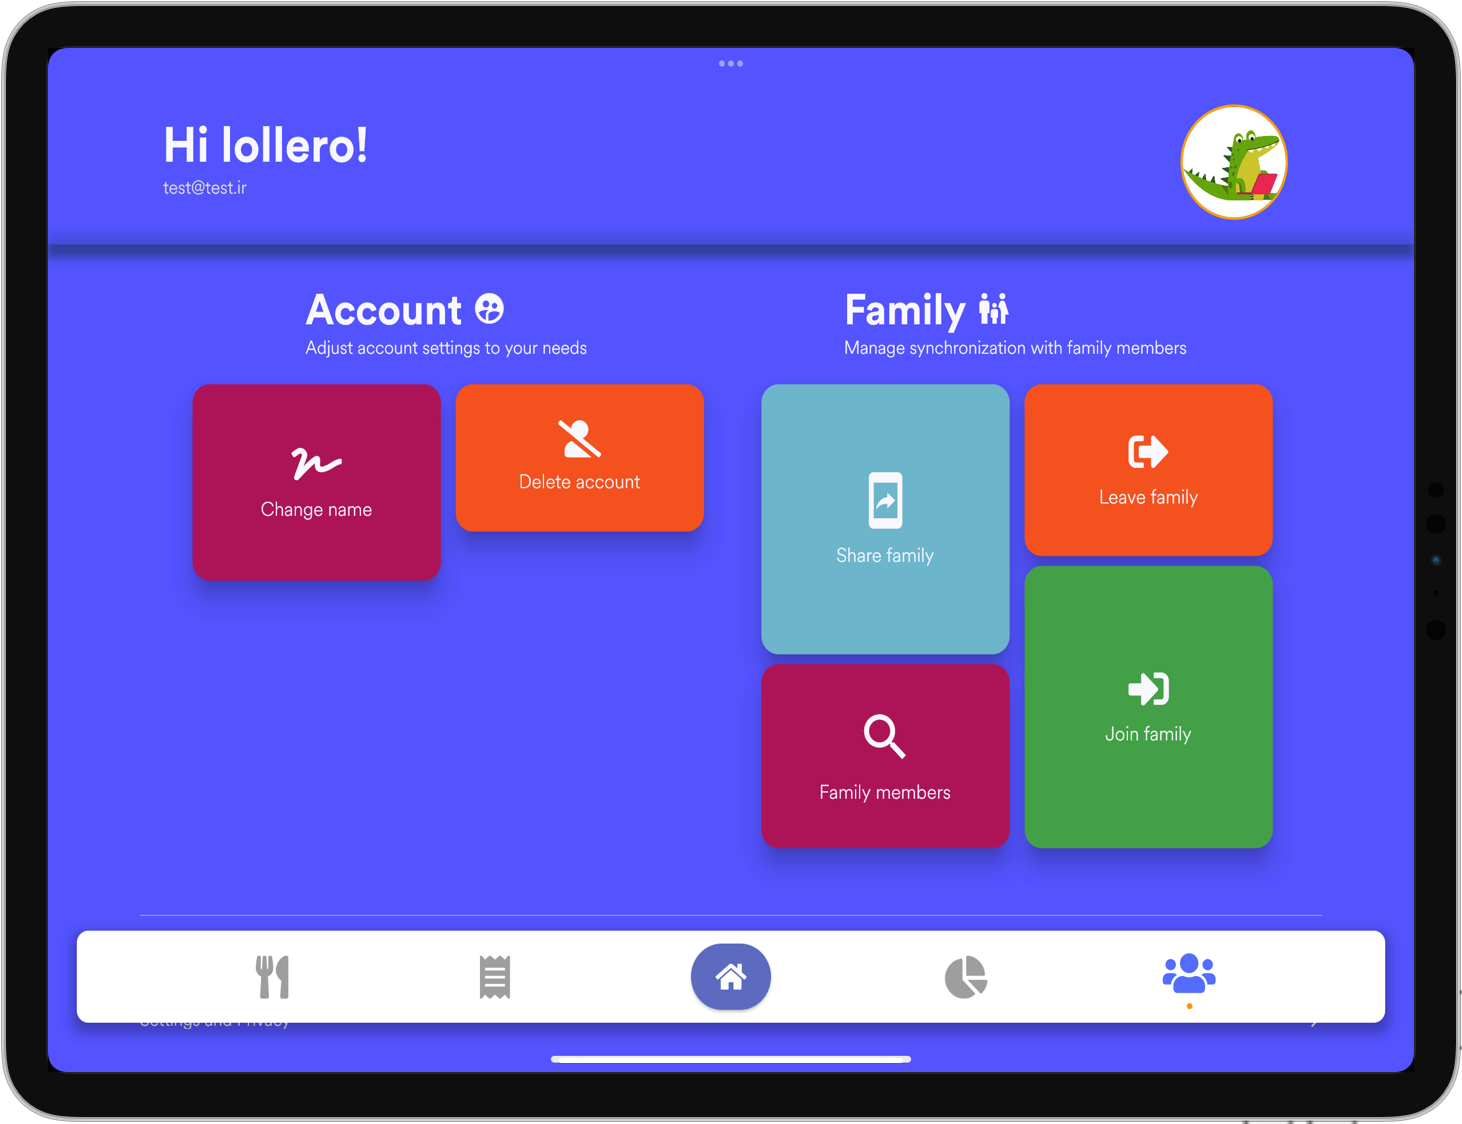
\includegraphics[scale=0.22]{./Images//Tablet_mocks/user1.png}
    \vspace*{-0.3cm}
    \caption{Tablet user info screen}
\end{figure}